\chapter{Improving QoE via Exploration and Exploitation at Scale}
\label{ch:pytheas}

%\newcommand{\Session}{\ensuremath{s}\xspace}
\newcommand{\Decision}{\ensuremath{d}\xspace}
\newcommand{\Quality}{\ensuremath{q}\xspace}
\newcommand{\Time}{\ensuremath{t}\xspace}
\newcommand{\SessionIndexi}{\ensuremath{{s_{i}}}\xspace}
\newcommand{\SessionIndexj}{\ensuremath{{s_{j}}}\xspace}
\newcommand{\DecisionIndex}{\ensuremath{d}\xspace}
\newcommand{\DecisionList}{\ensuremath{D}\xspace}
\newcommand{\HistoryList}{\ensuremath{H}\xspace}
\newcommand{\QualityMean}{\ensuremath{Q}\xspace}
\newcommand{\QualityVariance}{\ensuremath{C}\xspace}
\newcommand{\Feature}{\ensuremath{f}\xspace}
\newcommand{\FeatureSet}{\ensuremath{F}\xspace}
\newcommand{\FeatureIndexi}{\ensuremath{j}\xspace}
\newcommand{\FeatureValue}{\ensuremath{FV}\xspace}
\newcommand{\FeatureSetValue}{\ensuremath{FSV}\xspace}
\newcommand{\CF}{\ensuremath{CF}\xspace}

\renewcommand{\name}{{Pytheas}\xspace}
\providecommand{\mab}{{E2}\xspace}
\providecommand{\mablong}{{exploration and exploitation}\xspace}
\providecommand{\control}{{control}\xspace}
\providecommand{\idea}{{group-based \mab}\xspace}
\providecommand{\Idea}{{Group-based \mab}\xspace}

In the previous two chapters,
we have formulated the \ddn process as a
%Content providers are increasingly using data-driven
%mechanisms to optimize quality of experience (QoE).
%Many existing approaches formulate this process as a
prediction problem of learning optimal decisions (e.g.,
server, bitrate, relay) based on observed QoE of recent
sessions. While prediction-based mechanisms have
shown promising QoE improvements, they are necessarily
incomplete as they: (1) suffer from many known biases
(e.g., incomplete visibility) and (2) cannot respond
to sudden changes (e.g., load changes). Drawing a parallel
from machine learning, we argue that data-driven
QoE optimization should instead be cast as a real-time
exploration and exploitation (E2) process rather than as
a prediction problem. Adopting E2 in network applications,
however, introduces key architectural (e.g., how
to update decisions in real time with fresh data) and algorithmic
(e.g., capturing complex interactions between
session features vs. QoE) challenges. 

In this chapter, we present Pytheas,
a framework which addresses these challenges using
a group-based E2 mechanism. 
Inspired by the insight of persistent structures, we
observe that application
sessions sharing the same features (e.g., IP prefix, 
location) can be grouped so that we can run E2 algorithms
at a per-group granularity. This naturally captures
the complex interactions and is amenable to realtime
control with fresh measurements. Using an end-to-end
implementation and a proof-of-concept deployment
in CloudLab, we show that Pytheas improves video
QoE over a state-of-the-art prediction-based system by
up to 31\% on average and 78\% on 90th percentile of 
per-session QoE.

This chapter is organized as follows.
We begin with the limitation of prediction-based workflow (Section~\ref{sec:pytheas:limitations}) 
and why real-time \mab is a better abstraction
for \ddn (Section~\ref{sec:pytheas:casting}),
and then articulate key technical challenges for real-time \mab and outline the design rationale behind \name (Section~\ref{sec:pytheas:overview}).
We then present \name in more details from both algorithmic perspective (Section~\ref{sec:pytheas:algo}), and architectural (Section~\ref{sec:pytheas:system}) and an implementation perspective (Section~\ref{sec:pytheas:impl}).
Finally, we evaluate the performance of \name in Section~\ref{sec:pytheas:eval}, discuss related work in Section~\ref{sec:pytheas:related}, and summarize the section in Section~\ref{sec:pytheas:summary}.

\section{Limitations of Predictive Approaches}
\label{sec:pytheas:limitations}



\begin{figure}[t!]
\captionsetup[subfigure]{justification=centering,farskip=-1pt,captionskip=5pt}
\centering
%\hspace{-0.5cm}
\subfloat[Example A: Suboptimal quality due to fixed random data collection.]
{
        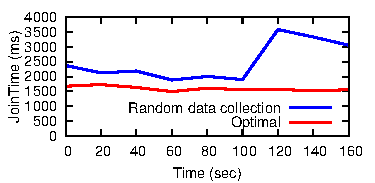
\includegraphics[width=0.45\textwidth]{figures/pytheas-problem-of-epsilon-change-JOINTIME.pdf}
        \label{subfig:problem-of-epsilon:change}
}
%\hspace{-0.1cm}
\subfloat[Example B: Overload and oscillations between decisions due to periodic prediction.]
{
        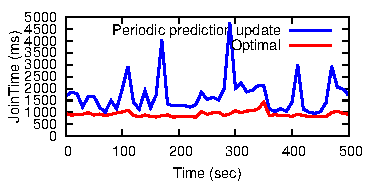
\includegraphics[width=0.45\textwidth]{figures/pytheas-problem-of-slow-load-JOINTIME.pdf}
        \label{subfig:problem-of-slow:load}
}
%\vspace{-0.2cm}
\caption{Limitations of prediction-oriented abstraction (e.g., CFA~\cite{cfa}) manifested in two real examples.}
%\vspace{-0.1cm}
\label{fig:abstraction}
\end{figure}


Many prior approaches (e.g.,~\cite{c3,cfa,cs2p,footprint}) 
for data-driven QoE optimization use a {\em prediction-based} 
workflow.  
That is, they periodically train a quality prediction model 
based on  passive measurements to inform decisions for 
future sessions; e.g., using history data to decide what 
will be  the best relay server for a Skype call or the best 
CDN for a video session?   
While such prediction-based approaches have proved useful, 
they suffer from well-known limitations, namely, 
{\em prediction bias} and {\em slow reaction}
~\cite{he2009learning,spand}.  
Next, we  highlight these issues using  CDN selection in 
video streaming as a concrete use case.% to highlight these effects.  

\subsection{Limitation 1: Prediction Bias}
A well-known problem of prediction-based workflows is that the prediction can be 
biased by prior decisions. Because the input measurement data are based on 
previous set of best decisions, we will 
not have a reliable way to estimate the potential  quality improvements 
of other decisions in the future~\cite{spand}.
%A simple measurement method is to passively measure the observed quality.
% Unfortunately, this  will bias future quality predictions as measurements will only be 
% based on the previous set of best decisions and we will 
%have to no reliable way to estimate the potential  quality improvements with other decisions in the future~\cite{spand}.
%\footnote{
% There could be other  systematic biases with passive measurements as well if there are hidden confounding factors. For instance, 
%  Google Hangouts uses relay servers only when a direct peer-to-peer connection is unavailable~\cite{hangouts-policy}. 
% However, sessions where the direct connection
% failed could have  intrinsically different behaviors (e.g., different connection types) from other sessions and thus estimating relay 
% performance from these measurements may provide incorrect predictions. }
A simple solution is to use a fixed percentage of sessions to explore 
different decisions. This could eliminate the above prediction bias.
However, it can still be suboptimal, since it might either let too many sessions  use suboptimal decisions when quality is stable, or collect insufficient data in presence of higher variance.

\smallskip \noindent\underline{Example A:}
Figure~\ref{subfig:problem-of-epsilon:change} shows a trace-driven evaluation to highlight such 
prediction biases. We use a trace of one of the major video providers in US. As a baseline, we consider prior work called CFA~\cite{cfa}, which uses a fixed fraction of 10\% sessions to randomly explore suboptimal decisions.\footnote{The process begins by assigning sessions uniformly at random to all decisions in the first minute, and after that, it assigns 90\% sessions to the optimal decisions based on the last minute.}
 We see that it leads to worse average video startup latency, or join time,
 than an optimal strategy that always picks the CDN with the best average quality in each minute.
Each video session can pick CDN1 or CDN2, and in the hindsight, CDN1 is on average better CDN2, except between t=40 and t=120,
 when CDN2 has a large variance.
 Even when CDN1 is consistently better than CDN2, CFA is worse than optimal, since it always assigns 10\% of sessions to use CDN2. 
 At the same time, when CDN2 becomes a better choice, CFA 
cannot detect this change in a timely fashion 
as  10\% is too small a fraction to reliably estimate quality of CDN2.

%Figure~\ref{fig:problem-of-epsilon} compares the quality of $\epsilon$-greedy with the optimal quality if we always pick the CDN with the best average quality.
%In Figure~\ref{subfig:problem-of-epsilon:stable}, CDN1 is constantly better than CDN2. 
%Since $\epsilon$-greedy always assigns 10\% of sessions to CDN2, quality of $\epsilon$-greedy is always substantially worse than optimal.
%In Figure~\ref{subfig:problem-of-epsilon:change}, CDN1 is better CDN2, except between 40 and 120 second, when CDN2 has a large variance and is better than CDN1.
%However, CFA could not identify the quality shift timely, because 10\% sessions are too few to reliably estimate quality of CDN2.
%In short, simple random data collection will either let too many sessions to use suboptimal decisions when quality is stable, or collect insufficient data when quality changes.

%\begin{figure*}[t!]
%\captionsetup[subfigure]{justification=centering,farskip=-1pt,captionskip=5pt}
%\centering
%\hspace{-0.5cm}
%\subfloat[Prediction-oriented abstraction]
%{
%        \includegraphics[width=0.35\textwidth]{figures/abstraction-prediction.pdf}
%        \label{subfig:abstraction-prediction}
%}
%\hspace{0.4cm}
%\subfloat[Real-time \mablong (\mab)]
%{
%        \includegraphics[width=0.35\textwidth]{figures/abstraction-mab.pdf}
%        \label{subfig:abstraction-mab}
%}
%\hspace{-0.5cm}
%\vspace{-0.1cm}
%\tightcaption{Comparing the traditional prediction-oriented abstraction with our abstraction of real-time \mab.}
%\vspace{-0.2cm}
%\label{fig:abstraction}
%\end{figure*}



\subsection{Limitation 2: Slow Reaction}
Due to the time taken to aggregate sufficient data for model building, 
today's prediction-based systems update quality predictions periodically on
coarse timescales; e.g., CFA updates models every tens of seconds~\cite{cfa}, and VIA updates its models every several hours~\cite{via}. 
%\cameraremove{\myparatight{Model drift}}
%Unfortunately, 
This  means that they cannot quickly adapt to changes in
operating conditions which can cause {\em model drifts}.  First, if there are
sudden quality changes (e.g., network congestion and service outage),
prediction-based approaches might result in suboptimal quality due to its slow reaction.  Furthermore, such model shifts might indeed be a
consequence of the slow periodic predictions; e.g., the best predicted server
or CDN will receive more requests and its performance may degrade
as its load increases.

\smallskip \noindent\underline{Example B:} We consider an AS and two CDNs. 
For each CDN, if it receives most sessions from the AS, it will be overloaded, and the sessions served by it will have bad quality.
Figure~\ref{subfig:problem-of-slow:load} shows that CFA, which always picks the CDN that has the best quality in the last minute, has worse quality than another
 strategy which assigns half of sessions to each CDN.  This is because 
 CFA always overloads the CDN that has the best historical performance by assigning most sessions to it, and CFA will switch decisions only {\em after} quality
degradation occurs, leading to oscillations and suboptimal quality.



At a high level,  these  limitations of prediction-based
approaches arise from the  logical
separation between measurement collection and decision making. Next, we discuss
what the right abstraction for data-driven QoE optimization should be to avoid
 these limitations.


\section{Casting QoE Optimization as a Exploration-Exploitation Process}
\label{sec:pytheas:casting}

To avoid these aforementioned limitations of prediction-based approaches, ideally we
want a framework  where decisions are updated in concert with measurement collection in real time.
%decisions and measurements are made in concert and
%updated in real time. 
%This could ideally  avoid unnecessary measurement collection, overloading decisions \vyas{vague},
% and adapt to flashcrowd swiftly.  
There is indeed a well-known abstraction in the
machine learning community that captures this---\mablong (\mab) 
processes~\cite{mab}.  Drawing on this parallel, we argue why   data-driven QoE
optimization should be cast instead as a {\em real-time \mab} process rather
than a prediction-based workflow.
%We begin by providing some brief background on \mab.
% 
% before showing how we cast  data-driven QoE optimization as 
% an \mab process (Figure~\ref{fig:casting}). 

%In contrast to the prediction-oriented abstraction% which predicts quality periodically by separately collected measurements (Figure~\ref{fig:abstraction-intro}(a)), 
%we take a first-principles approach and argue that the abstraction for data-driven quality optimization should be a {\em real-time \mablong (\mab)} process, where decisions and measurements are made in concert and updated in real time. 


%We use \mablong (or \mab), borrowed from machine learning literature, as a systematic formulation for \ddn problem. 
%\vyas{u need to do more handholding here -- what are teh two EEs etc}
\mypara{Background on \mablong} An intuitive way to visualize the \mablong (\mab) process is through the lens of 
a  multi-armed bandit problem~\cite{mab}.  Here, a gambler pulls
several slot machines, each associated with 
an unknown reward distribution.
The goal of the gambler is to optimize
the mean rewards over a sequence of pulls. 
 Thus, there is some intrinsic {\em exploration} phase where
 the gambler tries to learn these hidden reward functions, and subsequent  
{\em exploitation} phase to maximize the reward. Note that the reward 
 functions could  change over time, and thus this is a 
 continuous process rather than a one-time shot.
 
\mypara{QoE optimization as \mab (Figure~\ref{fig:casting})}  Given this framework,  we can see a natural mapping between \mab and data-driven QoE optimization.  
Like \mab, data-driven QoE optimization observes the QoE (i.e., reward) of a decision
every time the decision is used (i.e., pulled) by a session.
  Our goal is to maximize the overall QoE after a sequence of 
sessions.
%In \mab, each
%slot machine is associate with a reward distribution, an equivalent of each
%decision having some QoE distribution in data-driven QoE optimization.
%Moreover, both problems share the goal of optimizing overall rewards (QoE)
%within a limited number of pulls (or sessions).

Casting data-driven optimization as \mab not only provides 
a systematic framework for data-driven QoE optimization, 
but also allows us to leverage well-known algorithms (e.g.,~\cite{ucb1}) from the  machine learning literature.  
As \mab integrates the measurement collection (exploration) and 
decision making (exploitation) in a joint process,
we can dynamically explore decisions whose 
quality estimation has high uncertainty, and exploit decisions
that are clearly better.  For instance, in Example A, an \mab process could
 reduce traffic for exploration when QoE is stable (before 40
second and after 120 seconds), and raise it when QoE changes
(between 40 second and 120 second).  By running \mab in real time with the
most up-to-date measurement data, we could detect QoE drift as soon as some
sessions have experienced them, and adapt to them faster than
prediction-based approaches.  For instance, in Example B, real-time \mab
would detect load-induced QoE degradation on CDN1 as soon as its QoE is
worse than CDN2, and start switching sessions to CDN2 {\em before} overloading
CDN1.\footnote{Note that we do not need to know the capacity of each CDN, which is often unknown to content providers.}  
%Real-time
%\mab can also be robust to flash crowd. For instance, in Example C, if we
%detect the flash crowd as soon as it happens, we could separate sessions of the
%flash crowd and customize their decisions without affecting others.


 
%For instance, application quality vary over time, and to
%optimize quality under such time-varying distributions, we can borrow \mab
%techniques designed for non-stationary bandits (see more details in
%\Section\ref{subsec:??}).




\begin{figure}[t!]
\centering
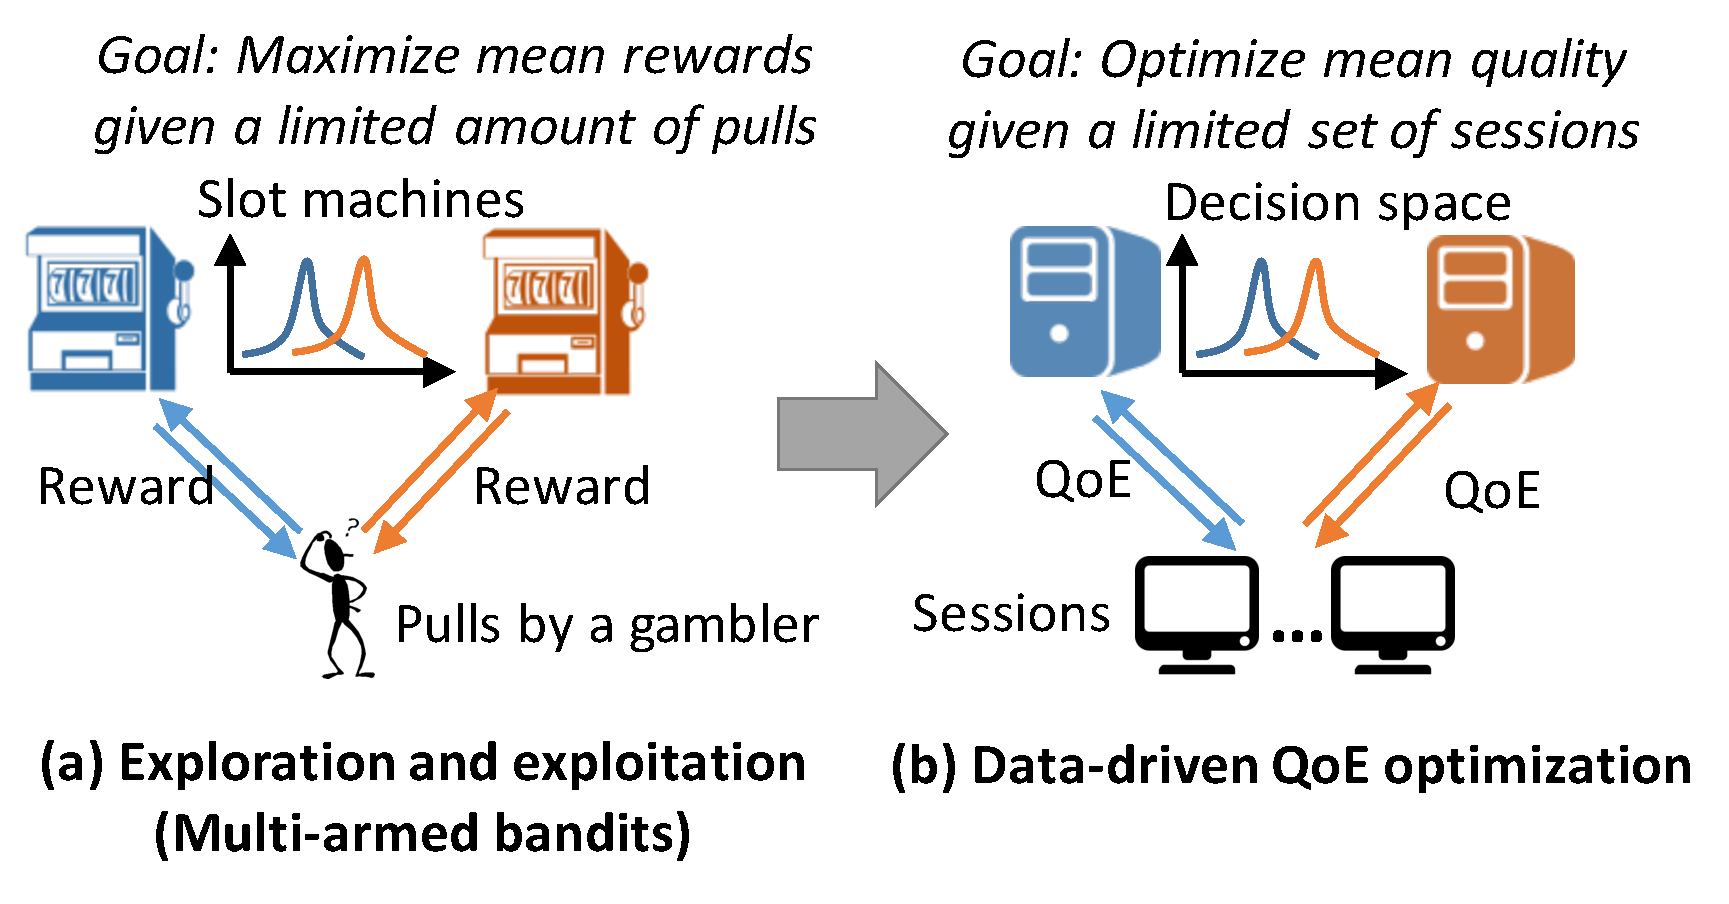
\includegraphics[width=0.7\textwidth]{figures/pytheas-casting.pdf}
%\vspace{-0.5cm}
\caption{Casting data-driven QoE optimization into formulation of \mablong (\mab).}
\label{fig:casting}
\end{figure}

\subsection{Challenges of E2 in the Networking Context}
While \mab offers the right abstraction in contrast to prediction-based approaches,
 applying it in network applications raises practical challenges:
\begin{packeditemize}
\item %{\em How to run real-time \mab over millions of globally distributed sessions with fresh data?} \\ 
%Running \mab at scale with real-time feedback is challenging, because 
Traditional \mab
techniques (e.g.,~\cite{mab,linucb,velox-cidr}) need fresh measurements of all sessions, 
but getting such a fresh and global view is challenging, because application providers
store fresh data in geo-distributed clusters, called {\em frontend clusters}, which only have a partial view across sessions.
Existing analytics framework for such geo-distributed infrastructure, however, either trade global view for
data freshness (e.g.,~\cite{c3}), or target query patterns of a traditional database (e.g.,~\cite{iris}), not
millions of concurrent queries from geo-distributed clients, as in our case.

%Unfortunately, many seemingly
%natural strawman solutions do not address this challenge.  For instance, split
%control architecture~\cite{c3} makes decisions by frontend clusters based on
%fresh data of the same session and stale data on other sessions.  It is
%reasonable to trade data freshness for scalability and responsiveness, when
%best decisions do not change often, but when quality or request pattern
%suddenly changes, split control will fall back to local adaptation, when
%multi-session view is needed the most to maintain desirable quality.
%Similarly, distributed data analytics platforms   store in geo-distributed
%clusters, but their existing solutions are not suitable for \ddn.  One approach
%assumes that data can be efficiently centralized in lower fidelity~\cite{??},
%but it is unclear how to reduce fidelity of quality measurements without
%letting \mab make suboptimal decisions.  Another approach performs analytics
%jobs in a distributed way and aggregates results in real time~\cite{??}, which
%is suitable to handle tens of requests per second, but it is not desirable to
%update \mab decisions for millions of sessions. \vyas{too much text and noise.
%please shrink}



%To guarantee responsiveness to globally distributed
%clients, application providers have deployed geo-distributed frontend
%clusters~\cite{??,??}, so that the user activities and logs (including quality
%measurements) are first stored in frontend clusters and periodically archived
%to a backend on coarse timescale of minutes or hours~\cite{c3} and often in
%lower fidelity~\cite{jetstream}.  Therefore, neither frontend nor backend
%provides a fresh and global view of measurements needed by \mab algorithms.

%First, we need to a system architecture that updates the \mab decision in real time with the most up-to-date measurement data, and responds to client requests very quickly.
%This is challenging, because \mab techniques (e.g.,~\cite{linucb,velox}) need fresh and global view of measurement data, whereas service providers store fresh client data in geo-distributed clusters, each having only a partial view.
%To serve globally distributed clients, application providers today have deployed geo-distributed frontend clusters~\cite{??,??} so that the
%user activities and logs (including quality measurement) are first stored one of clusters and periodically updated to a backend on coarse timescale of minutes or hours and often in lower fidelity. 
%This makes it difficult to maintain a fresh view of all data to update MAB decision, as it takes time to gather the sheer size of measurement data from different frontend clusters to where decisions are made. 
%Such situation would even be common, if contextual MAB algorithm (e.g.,~\cite{linucb,velox}) needs a global view of measurement data to make decisions.
%For instance, even though MAB techniques can react fast enough in theory where decision is updated with the most recent feedback, their reaction speed would be bottlenecked by the existence of substantial feedback delay.


%\vspace{0.1cm}\noindent{\bf How to model networking ``context'' in MAB?}
\item %{\em How to model ``network context'' in \mab?}\\
Traditional \mab techniques also make strong assumptions about the context
that affects the reward of a decisions, but they may not hold in network settings.
For instance, they often assume some notion of
continuity in context (e.g.,~\cite{cmab}), but even when some video sessions match on
all aspects of ISP, location, CDN resource availability, they 
may still see very different QoE, if they differ on certain key feature 
(e.g., last-hop connection)~\cite{cfa}.

%Network sessions with different network contexts (e.g., last-mile connections, WAN performance,
%CDN resource availability, and device information) should not be treated identical in an \mab process.
%One option is to use so called ``contextual multi-armed
%bandit''~\cite{cmab} techniques, where rewards of a
%bandit also depends on the context of a certain pull, but they often assume some notion of
%continuity in context, but two network sessions that match on all features
%except one can still have very different network performance~\cite{cfa}.

%Application sessions with different network ``contexts'' do not share same
%optimal decisions, so \mab process should be aware of the network context,
%rather than treating all sessions identically.  For instance, video quality
%depends on complex factors including last-mile connections, WAN performance,
%CDN resource availability, and device information, and sometimes, their
%combinations~\cite{cfa}, so the degree to which one session's quality should
%affect the selection of CDNs, bitrate, or network path of another session
%varies greatly across sessions.  One option is to use ``contextual multi-armed
%bandit''~\cite{??} techniques from \mab literature, which assumes rewards of a
%bandit depends on the context of a pull, but they often assume some notion of
%continuity in context; e.g., similar contexts always yield similar
%rewards~\cite{??}, whereas two network sessions that match on all features
%except one can still have very different network performance~\cite{cfa}.
%Alternatively, we can use more domain-specific techniques
%(e.g.,~\cite{cfa,cs2p}), but they are designed for quality prediction.  For
%instance, CFA uses critical features to mode sessions with similar quality, but
%critical features do not indicate whether a session should explore different
%decisions to optimize the quality for future sessions.
% \vyas{too much text and noise.
%please shrink - not more than 5-6 lines for each challenge}



\end{packeditemize}


%For instance, CFA only predicts for each session which decision should be exploited under contextual settings, but it does not decide when it should be used to explore different decisions.

%CMAB techniques, however, are no panacea, especially in a networking context. 

%\begin{packedenumerate}
%\item Need for context: quality distributions differ across sessions.
%\item Contextual MAB requires domain-specific modeling of the context.
%\end{packedenumerate}



%\begin{packedenumerate}
%\item MAB cannot react fast (even though it logically can), if the feedback delay is on timescale of minutes.
%\item It's challenging for existing architecture to achieve required feedback delay for MAB.
%\end{packedenumerate}












\section{Overview of Pytheas Ideas}
\label{sec:pytheas:overview}

%In a general setting, the combination of the above challenges 
% might make \mab intractable. However, 
To address the practical challenges of applying \mab in network applications, 
we observe a key domain-specific insight in networked applications
 that enables us to address both challenges in practice. We highlight the intuition 
 behind our insight, which we refer to as \idea, and then provide an overview of the \name system 
 which builds on this insight.  

%called \idea, inspired by the insight that sessions with
%similar context are often nearby in terms of geographical location and IP
%space, and can be grouped.

\mypara{Insight of  \Idea}
Our insight is that the ``network context'' of application sessions is often aligned with
their ``network locality''.
That is, if two sessions share the context that determines their \mab decisions, 
they will be likely to match on some network-specific features.
We see manifestations of this insight in many settings.
% When clients share certain location or IP prefix-related
%features, they are more likely to have the similar video QoE~\cite{cfa} and
%similar TCP throughput~\cite{cs2p,spand} at the same point of time. 
 For instance, video
sessions with similar QoE from the same CDN/server tend to match on 
client IP prefix~\cite{cfa,cs2p}. 
Similarly, VoIP calls between the same ASes are likely to share the best
relays~\cite{via},  and clients from  same /24 IP prefix will have
similar web load time from the same edge proxy~\cite{footprint}.
In Section\ref{subsec:frontend}, we validate this insight with a real-world dataset.

%This insight suggests two natural implications:
%\begin{packeditemize}
%
%\item First, a global view is not necessary to run \mab for network applications.
%
%\item Second, when a session queries a frontend cluster for decision, the same cluster is likely to receive the data of other sessions in the same group.
%\vyas{this is still bad. the notion of frontend etc has not been defined!}
%
%\end{packeditemize}
%
%\vyas{there seems to be two insights --- group based ee can be done and these groups goto same frontend? but the 
% above insight doesnt imply they will get mapped to same frontend. also it might be cleaner to difrectly go below than this 
% indirect step}


%\begin{packeditemize}
%
%\item First, the \mab context of sessions has natural ``boundaries''.
%%\vyas{dont follow this cliff thing!}
%For instance, if two sessions share a performance bottleneck, they will be much more likely to share the same network context that affect their \mab decisions than otherwise. 
%In other words, it is not a necessary condition that \mab process needs a global view of QoE of all sessions.
%%We see such effect manifest itself in various applications, such as critical features in video streaming~\cite{cfa}, Internet telephony~\cite{via}, and web application sessions~\cite{??}.
%
%\item Second, sessions with similar \mab context are often in the same geographical locations and IP space.
%For instance, QoE of a video session is often critically determined by ASN~\cite{cfa}, which means video sessions sharing similar \mab context are likely in the same ASN.
%%Similar observations has also been made in TCP performance~\cite{spand}, Internet telephony~\cite{via}, and web application sessions~\cite{??}.
%
%\end{packeditemize}
%We see manifestations of both effects in a variety of applications.
%When clients share certain location or IP prefix-related features, they are more likely to have the similar video QoE~\cite{cfa} and similar TCP throughput~\cite{cs2p,spand} at the same point of time.
%Video sessions share similar QoE if the match location or IP prefix-related features~\cite{cfa}.
%Two Internet telephony calls are likely to share the best relay option when they have the same peering points with the relay services~\cite{via}.
%Users with same /24 IP prefix are very likely to have similar web load time from the same proxy or data center~\cite{footprint}.


This insight inspires the notion  of {\em \idea}, which can 
 address the above challenges by enabling an effective decomposition 
 of the \mab process (Figure~\ref{fig:system-overview}a).  
 Specifically, instead of a global \mab
process over all sessions, we group together sessions with similar context by 
network locality and other key features (such as device and location), and
use one \mab process for each group.
% It addresses the challenges of real-time
%\mab for two reasons:
%\begin{packeditemize}
%\item 
Since sessions within a group share network locality (e.g., 
in the same locations and IP prefixes), 
they are likely to be mapped to the same frontend cluster.
By running the per-group \mab logic in this frontend cluster, we can update
decisions with fresh data from other sessions in the group received by this frontend cluster.
%\item 
 Furthermore, as each group consists of sessions with similar context, 
it is sufficient to use traditional \mab techniques based on the data of sessions
in one group, 
without needing a global view of all sessions.
%\end{packeditemize}
It is important to note that sessions are not grouped entirely based on IP prefixes. The sessions in the same network locality could have very different QoE, depending on the device, last-hop connectivity, and other features. Therefore, we group sessions on a finer granularity than IP prefix.

\begin{figure}[t!]
\centering
%\includegraphics[width=0.5\textwidth]{figures/system-overview.pdf}
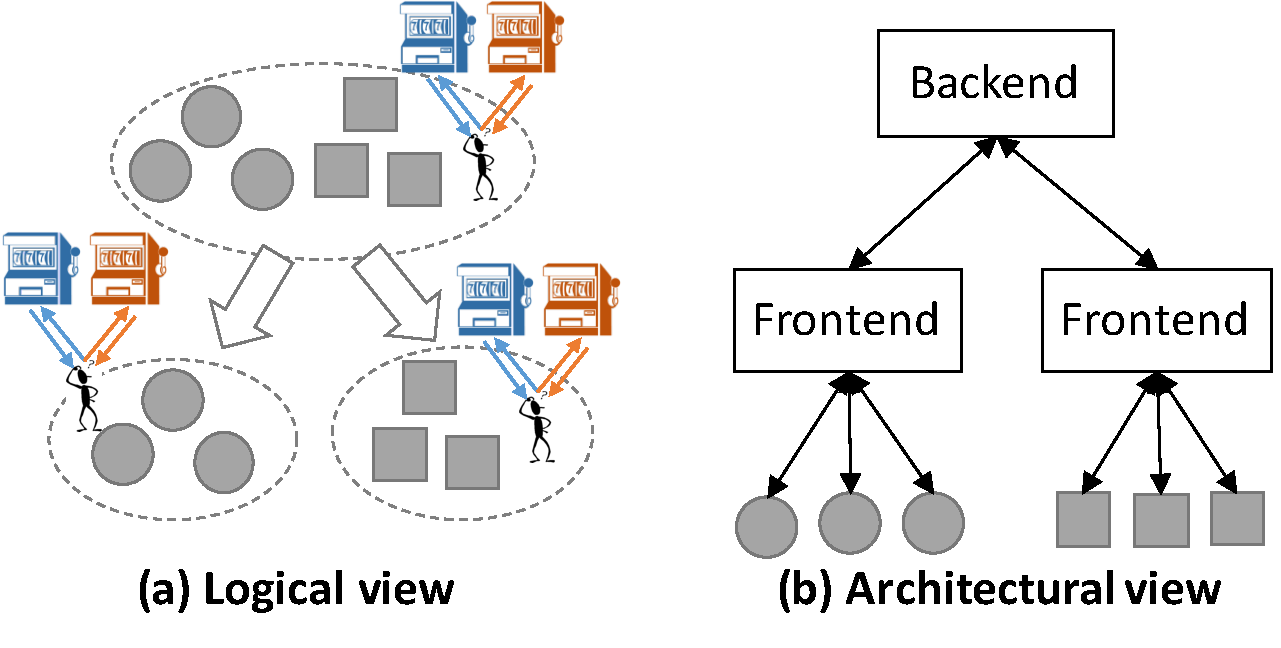
\includegraphics[width=0.6\textwidth]{figures/pytheas-system-overview-group.pdf}
%\vspace{-0.4cm}
\caption{Illustration of \idea.}
%\vspace{0.1cm}
\label{fig:system-overview}
\end{figure}



\mypara{System overview}
Figure~\ref{fig:system-overview}b shows how the \idea is realized in the \name architecture.
Each session group is managed
by one per-group \mab process run by one frontend cluster.  When a session
comes in, it sends a request for its control decisions, which includes its features,
to the \name system.  The request will be received by a frontend
cluster, which maps the session to a group based on its features, then
gets the  most up-to-date decision from the local per-group \mab process, and
returns the decision to the session.  Each  session measures its QoE and reports it  to the same frontend cluster.  When this frontend
receives the QoE measurement, it again maps the session to a group, and
updates the \mab logic of the group with the new measurement.  
In most cases, the
\mab logic of a group is run by the same cluster that 
receives the requests and
measurements of its sessions, 
so \mab logic can be updated in real time. 

%When the frontend cluster receives the control requests from another session
%in the same group, it returns the fresh decision made by the local \mab
%process.
%Nonetheless, when sessions of a group  are received by different clusters 
%(e.g., the ``square'' sessions in Figure~\ref{fig:system-overview}b), one of
%them will be picked to run the per-group \mab logic, and other clusters will
%cache the decisions and forward QoE measurements in a near real-time
%fashion.

%Note that multiple \mab processes can run in the same frontend cluster, and one group can span across multiple frontend clusters. 

 The backend cluster has a global, but
slightly stale, view of QoE of all sessions, and it determines the session
groups -- which group each session belongs to and which frontend should run
the per-group logic for each group.  Normally, such grouping is updated
periodically on a timescale of minutes. During sudden changes such as frontend cluster failures, it can also be triggered on demand to re-assign groups to frontend clusters.

%\camera{On a high level, group-based \mab addresses the challenges of applying \mab in network applications through (1) modeling ``network context'' by grouping session sharing QoE-determining factors, and (2) realizing real-time \mab by running control logic in the frontend clusters while learning the slow changing session groups in the backend cluster.}

The following sections will present the algorithms (Section~\ref{sec:pytheas:algo}) and system design (Section~\ref{sec:pytheas:system}) of \name, and how we implemented it (Section~\ref{sec:pytheas:impl}) in more details.


%\subsection{Running example}
%
%This part gives a simple running example to show the workflow of \name.




\section{Pytheas Algorithms}
\label{sec:pytheas:algo}


Using \idea, \name decouples real-time \mab into two parts:
a {\em session-grouping} logic to partition sessions into groups, and a {\em per-group \mab} logic
that makes per-session decisions. This section presents the design of these two core 
algorithmic pieces and how we address two issues:\footnote{We assume in this section that the per-group control logic is updated in real time (which will be made possible in the next section).} 
(i) Grouping drift: the session-grouping logic should dynamically regroup sessions based on the context that determines their QoE; 
and (ii) QoE drift: the per-group control logic should switch decisions when QoE of some decisions change. 



\subsection{Session-Grouping Logic}
\label{subsec:grouping}

Recall that sessions of the same group share the same factors on which their
QoE and best decisions depend.  As a concrete example, let us consider  CDN
selection for video.  Video sessions in the same AS whose QoE depends on the
local servers of different CDNs should be in the same group. However, video
sessions whose QoE is bottlenecked by home wireless and thus is independent to
CDNs should not be in the same group.  In other words, sessions in the
same group share not only the best decision, but also the factors that
determine the best decisions.

 A natural starting point for this grouping decision is 
 using the notion of critical features proposed in prior work~\cite{cfa}.  At a high level,
 if session A and B have the same values of  critical features,
 they will have similar QoE. 
% In the particular model, the space of decisions 
% (e.g., CDN, bitrate) is  simply another session feature.
Let  $\mathit{S}(s,F,\Delta)$ denote the 
  set of sessions that occur within the last $\Delta$ 
 time interval and share the same  feature values as $s$ on the set of features $F$, and 
 let $Q(X)$ denote the QoE distribution of a session set $X$. 
Then, the critical feature set $F^*$ of a session $s$:
%by the feature subset $F$ of $F^{all}$, such that 
\begin{displaymath}
\textrm{argmin}_{F\subseteq F^{\mathit{all}},  |S(s,F,\delta)| > n} | Q(S(s,F^{\mathit{all}},\Delta)) - Q(S(s,F,\Delta))| 
\end{displaymath}
% That is,  using  the 
% historical measurements matching just  $F^*$, we have a good  prediction of  the quality of the session $s$
% in the past over the $\Delta$ time interval (say last hour).
That is, the historical session who match values on critical features $F^*$ with $s$ 
have very similar QoE distribution to those matching on all features with $s$ on a 
long timescale of $\Delta$ (say last hour).
 The   clause $|S(s,F,\delta)| > n$  ensures that  there is sufficient mass in that set 
 to get a statistically significant estimate even on small timescales $\delta$ (e.g., minutes). 
%minimizes the difference between the QoE
%distributions of sessions which match on $F^{all}$ with $s$ in the last hour)
%and that of sessions $Q^{LastHour}(s,F)$ (which match on $F$ with $s$ in the last hour), and
% there are enough sessions matching on $F$.
 Such a notion of critical features has also been (implicitly) used in many other
applications; e.g., AS pairs in VoIP~\cite{via} and 
 /24 prefixes for web page load time~\cite{footprint}.
 Thus,  a natural strawman for grouping algorithm is to groups sessions who match on their critical features,
 i.e., they have similar QoE.
  

However, we observe two  problems inherent to critical features, which make
it unsuitable to directly group sessions based on critical features:
(1) First, grouping sessions based on critical features may result in groups that consist of
only sessions using similar decisions, so their measurement will be biased towards a subset of decisions.
(2) Second, grouping sessions based on critical features will also create overlaps between groups, so 
\mab logic of different groups could make conflicting decisions on these overlapping sessions.
%because when session $s_1$ matches its critical features with $s_2$, 
%$s_2$ may have a different set of critical features to $s_1$.
For instance, consider two Comcast sessions, $s_1$ and $s_2$, if the critical feature of $s_1$ is ISP, 
and the critical feature of $s_2$ is its local WiFi connection, 
$s_2$ will be in both the ``WiFi'' group and the ``Comcast'' group. 

%Realizing the similarity and fundamental difference between critical features and session grouping, 
To address these issues, we formulate the goal of session grouping as following.
Given a session set, the session-grouping logic should output any non-overlapping partition of sessions 
so that if two sessions $s_1$ and $s_2$ are in the same group, $s_1$ and $s_2$ should 
match values on $s_1$ or $s_2$'s non-decision-specific critical features. 
Non-decision-specific features are the features independent of decisions; e.g., ``device'' is a feature independent of decisions, since video sessions of the same device can make any decisions regarding CDN and bitrate.

Operationally, we use the following approach to achieve such a grouping.
First, for each session, we learn its critical features, and then ignore decision-specific features from the set of critical features of each session.
%Then, we group sessions so that 
%and then assigning overlapping parts to one of the overlapping groups.
%For instance, if B and C's groups overlap on A, we can simply assign A to B's group (or C's group), because the decision of A will not affect the logic of C's group, if A is in B's group.
%Note that this could lead to smaller groups than all sessions sharing values on their critical features, but as we will see in \Section\ref{sec:eval}\jc{Don't forget to result the results}, most sessions are in the groups with sufficient amount of sessions.
Then, we recursively group sessions based on the remaining critical features in a way that avoids overlaps between groups.
We start with any session $s_1$, and create a group consisting of all sessions that match with $s_1$ on $s_1$'s critical features.
We then recursively do the two following steps until every session is in some group.
We find a session $s_2$, who is not included in any existing group, and create a new group of all sessions that match with $s_2$ on $s_2$'s critical features.
If the new group does not overlap with any existing group, it will be a new individual group, otherwise, we will add it to the existing groups in the way illustrated in Figure~\ref{fig:grouping-example}.
%Figure~\ref{fig:grouping-example} shows how non-overlapping groups can be created by incrementally adding new groups based on critical features.
%At any point, 
We organize the existing groups in a graph, where each node is split by values of a certain feature, and each group includes multiple leaf nodes.
For instance, if we want to add a new group that consists of sessions whose ``content'' is ``Super Bowl'' to a graph of existing groups as shown in Figure~\ref{fig:grouping-example}a, we will fork a path to create a new leaf node whenever the new group overlap with a existing group.
Note that, this means multiple leaf nodes may be belong to the same group (e.g., ``Group 3'' in Figure~\ref{fig:grouping-example}b contains two different leaf nodes).

%The session-grouping logic also handles grouping drifts caused by sudden changes in workload, such as flashcrowd. We will be discuss it in \Section\ref{subsec:flashcrowd}.

%\camera{The session-grouping logic also will dynamically regroup sessions to handle frontend failure. We will discuss it in \Section\ref{subsec:fault}.}

%
%\vyas{here is the structure of this:
%
%1. Start with CFA formula of mathematical problem that CFA is solvng \\
%
%2. Then say here are two key reasons why it wont work -- a. it includes decision b. it can overlap \\
%
%3. Intuitively how to fix a/b \\
%
%4. What does group formula look like for the mathematical problem  \\
%}



%Note, however, \mab has different requirement than QoE prediction, which
%renders critical features not directly useful.  At first glance, we could group
%sessions who match on critical features, but this will create overlaps between
%groups, over which \mab logic of different groups could make conflicting
%decisions. Consider that session A matches on its critical feature with B and
%C, but session B and C do not match on their critical features. While this is
%allowed for QoE prediction, in \idea, the logic of B's group and that C's group
%might make different decisions for A. 


\begin{figure}[t!]
\centering
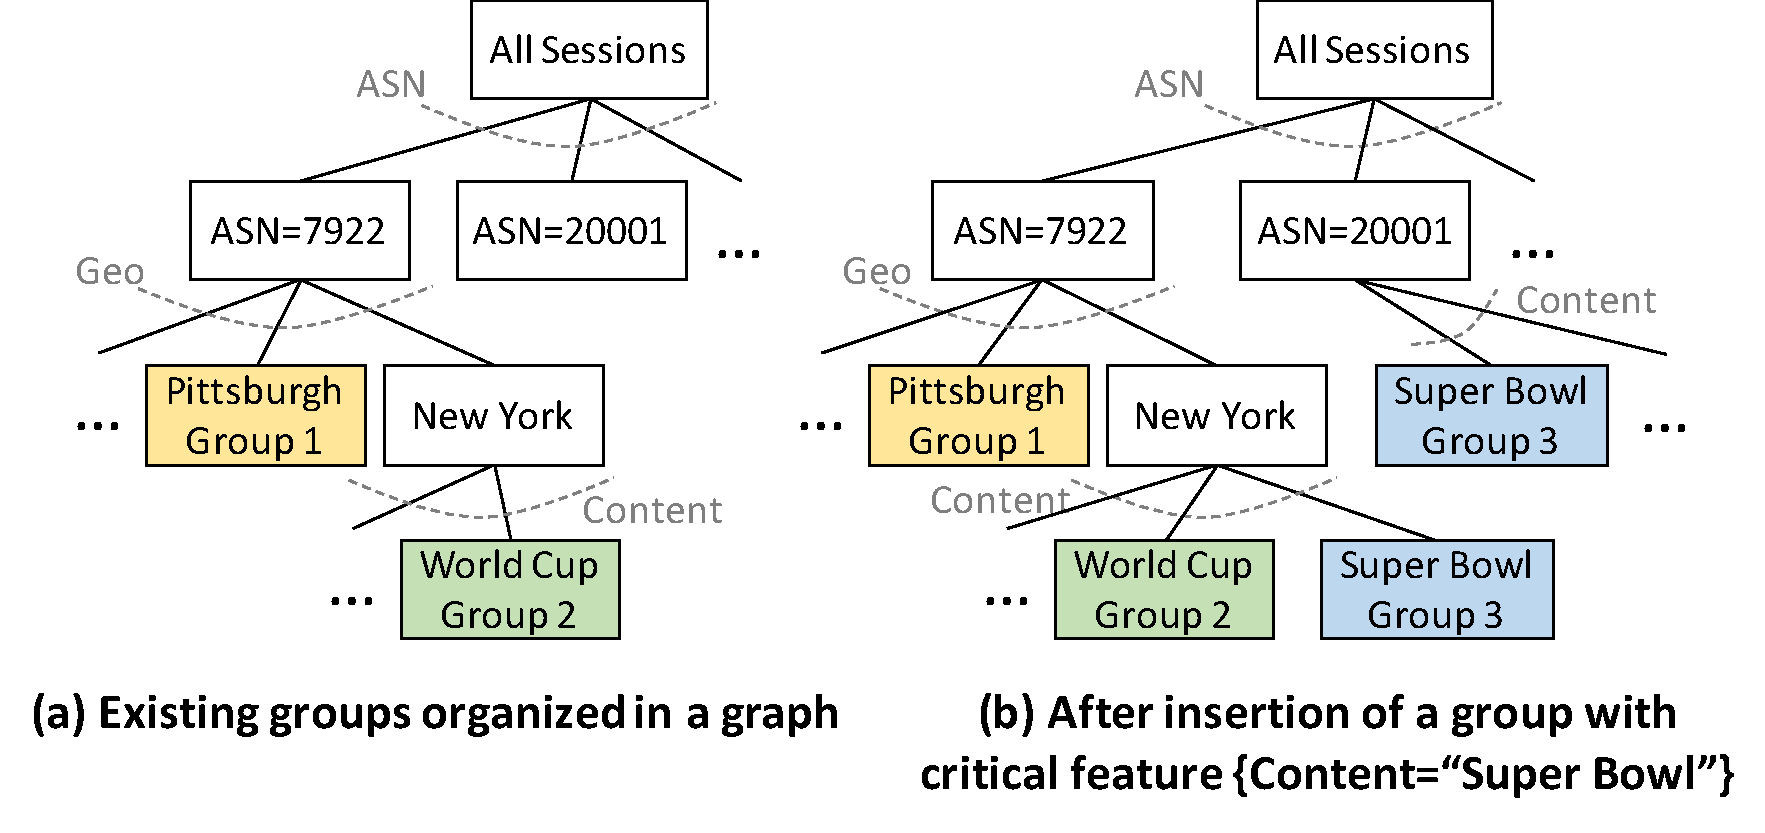
\includegraphics[width=0.85\textwidth]{figures/pytheas-grouping-example-2.pdf}
\caption{An illustrative example of session groups organized in a graph and how to a new group is added.}
\label{fig:grouping-example}
\end{figure}







\subsection{Per-Group \mab Logic}
\label{subsec:per-group}

To run \mab in presence of QoE drift, we use Discounted UCB
algorithm~\cite{discounteducb}, a variant of the UCB algorithm~\cite{ucb1}, as the
per-group \mab logic.  UCB (Upper Confidence Bound) algorithms~\cite{ucb1} are a
family of algorithms to solve the multi-armed bandits problem.  The core
idea is to always opportunistically choose the arm that has the highest
upper confidence bound of reward, and therefore, it will naturally tend to
use arms with high expected rewards or high
uncertainty. Note that the UCB algorithms do not explicitly assign sessions 
 for ``exploration'' and ``exploitation''.

We use Discounted UCB algorithm to adapt to QoE drift, because it automatically
gives more weight to more recent measurements by exponentially discounting
historical measurements.  Therefore, unlike other UCB algorithms which will
(almost) converge to one decision, Discounted UCB is more likely to revisit
suboptimal decisions to retain visibility across all decisions.
%As details of Discounted UCB can be found in~\cite{discounteducb}, we describe
%only its high level intuition here.  
We refer readers to~\cite{discounteducb} for more details.
Given a session $s$, it
returns a decision that has not been tried, if there is any.  Otherwise, it
calculates a score for each potential decision $\DecisionIndex$ by adding up an
exponentially weighted moving average of $\DecisionIndex$'s history QoE and an
estimation on the uncertainty of reward of $\DecisionIndex$, and picks
the decision with highest score.


%\vyas{is there any "adaptation" or extension of the algorithm to this context? if
% so try to highlight that} 


%$\bar{\QualityMean}(\gamma,\DecisionIndex)+{\QualityVariance}(\gamma,\DecisionIndex)$.
%Here, $\bar{\QualityMean}(\gamma,\DecisionIndex)$ is an exponentially weighted moving average of QoE of history sessions that used $\DecisionIndex$, 
%and ${\QualityVariance}(\gamma,\DecisionIndex)$ is an estimation on the uncertainty of reward of $\DecisionIndex$.
%By default, we use $\gamma=0.9$, which has good empirical performance.





\section{Pytheas System Architecture}
\label{sec:pytheas:system}

%Having an algorithmic framework of MAB is half of the story.
%To run the logic for per-group control and session grouping at scale, we seek a system design that meets three goals:
Given the algorithmic pieces from the previous section, next 
we discuss how we map them into a system architecture.
  At  a high level, the \mab logic of each group is independently run by frontend clusters,
while the session-to-group mapping is continuously updated by the 
backend.

%\vyas{i dont get any sense of what to expect in this section}

\subsection{Requirements} 
 The \name system design must meet four goals:
\begin{packedenumerate}
\item {\em Fresh data:} The per-group \mab logic should be updated every second with newest QoE measurements.
\item {\em Global scale:} It should handle millions of geo-distributed sessions per second.
\item {\em Responsiveness:} It should respond to requests for decisions from sessions within
 a few  milliseconds.
\item {\em Fault tolerance:} QoE should not be significantly impacted when parts of the system fail.
\end{packedenumerate}

%\tightsubsection{Split control vs. \idea}

%\vyas{dont start with this .. no one knows what split control is!!}
%\vyas{as written it sounds more incremental wrt C3 than it really is!}
%\vyas{not even sure why 6.1 is necessary. i can just move it to related work}

%It is helpful to understand the architectural benefit of \idea by contrasting
%it with split control.  

A natural starting point to achieve this goals might be to adopt a ``split
control plane'' approach advocated by prior work for prediction-based 
approaches~\cite{c3,cfa}.  At a high level, this split control plane has two parts: (1)
a backend cluster that generates centralized predictions  based on  global but
stale data, and (2) a set of geodistributed frontend servers  that use these predictions
from the backend to make decisions on a per-session basis.  
%In addition,  the clients also run per-session adaptation
%algorithms as fall back strategies.  
This split control architecture  achieves  global  scale and
high responsiveness, but fundamentally sacrifices data freshness.  
%While this
%tradeoff was inevitable in the prediction-oriented abstraction adopted by prior
%work~\cite{c3,cfa}, this violates the requirements of running \mab processes.


 \name  preserves the scale and responsiveness of the split control
approach, but extends  in  two key ways to run  \idea with fresh data. First,
each frontend cluster runs  an active \mab algorithm rather than merely
executing the (stale) prediction decisions as in prior work.  Second, the
frontend clusters now run per-group logic, not per-session logic.  This is
inspired by the insight that sessions in the same group are very likely to be
received by the same frontend cluster.  Thus, \idea could achieve high data
freshness on the session group granularity, while having the same scale and
responsiveness to split control.
Next, we discuss the detailed design of the frontend and backend 
 systems. 
 
%  the dper-session decision execution algorithm 
%he \idea architecture used in \name is similar to split control but with a key
%difference: 

 
%To achieve scalability and responsiveness, split
%control performs per-session control logic at frontend clusters, while using
%the backend cluster to make centralized hint based on the global yet stale
%data.  

\subsection{Per-Group Control by Frontends}
\label{subsec:frontend}


The best case for \idea is when all sessions of the same group are received by
the same frontend cluster.  When this is true, we can run the per-group \mab
logic (Section~\ref{subsec:per-group}) in real time with fresh measurements of
the same group.  In fact, this also is the common case.  To show this, we ran
session-grouping logic (Section~\ref{subsec:grouping}) on 8.5 million video
sessions in a real-world trace, and found around 200 groups each minute. Among these groups, we found that (in
Figure~\ref{fig:fraction-same-frontend}) for 95\% of groups, all sessions are
in the same AS, and for 88\% of groups, all sessions are even in the same AS
{\em and} same city.  Since existing session-to-frontend mappings (e.g., DNS or Anycast-based mechnisms) 
are often based on AS
and geographical location, this means that for most groups, their sessions will
be verly likely to be received in the same frontend clusters.

%This means when a per-group logic receives a decision request, all data it needs are received by the same cluster, so the per-group control logic can be updated with in real time with fresh per-group data.


\begin{figure}[t!]
\centering
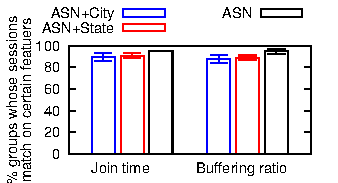
\includegraphics[width=0.45\textwidth]{figures/pytheas-Eval-fraction-same-frontend.pdf}
%\vspace{-0.2cm}
\caption{For most groups, the sessions are in the same ASN and even same city.}
\label{fig:fraction-same-frontend}
\end{figure}

 In practice, however, it is possible that sessions of one group are spread across 
frontend clusters.
%\footnote{We take a pragmatic stance that each session request or
%measurement is directed by one of many geo-distributed frontend clusters via
%DNS or anycast services, like in most today's service providers. Such
%redirection services are usually shared with critical real application traffic,
%so we assume \name does not have control over how a client is redirected to the
%frontend clusters.}
 We have two options in this case:
\begin{packedenumerate}
\item Pick one cluster as the {\em leader} cluster of this group and let it run the \mab logic of the group based on the measurements received by this cluster. Meanwhile, other clusters, called {\em proxy} clusters of the group, simply receive decisions periodically from the leader cluster.
\item Keep the leader cluster and proxy clusters, but let proxy clusters not only receive decisions from the leader, but also forward QoE measurements to the leader cluster.
\end{packedenumerate}
We see a tradeoff between the two options.
While Option 1 is less complex to implement than Option 2, the leader proxy in Option 1 runs per-group logic based on only a subset of sessions, especially when the sessions of a group are evenly spread across many frontend clusters.
We pick Option 2, because it is cleaner in that the per-group logic is based on all sessions in a group. In fact, implementing Option 2 does not add much complexity.
Finally, Option 2 can easily fall back to Option 1 by stop forwarding measurements from proxy clusters to the leader cluster.





\subsection{Updating Session Groups in the Backend}
\label{subsec:backend}

%The role of the backend in group-based control is two-fold.
The backend cluster uses a global, stale view of measurements to update two tables, which are sent
 to the frontend to regroup sessions.
\begin{packeditemize}
\item First, the backend runs the session-grouping logic (Section~\ref{subsec:grouping}) to decide which group each session belongs to, and outputs a {\em session-to-group table}.
\item Second, it decides which frontend should be the leader cluster of each group and outputs a {\em group-to-leader table}. For each group, we select the frontend cluster that receives most sessions in the group as the leader.
\end{packeditemize}
%For each group, we select the frontend cluster that receives most sessions in the group, because this will minimize the number of sessions in the proxy clusters, whose decisions and measurements need to be shared across frontend clusters.
%To this end, each frontend cluster will count the number of sessions each group receives, and sends these counts to the backend.
The backend periodically (by default, every ten minutes) updates the frontend clusters with these two maps.  
%\cameraremove{The only exception when the maps are updated in
%near real time is when flash crowd happens, which will be discussed in the next
%section.}
The only exception for the maps to be updated in
near real time is when one or more frontend clusters fail, which we discuss next.



%\cameraremove{
%\tightsubsection{Handling flash crowds}
%\label{subsec:flashcrowd}
%}
%
%\cameraremove{
%Session groups tend to change slowly, except when flash crowd happens.
%Unlike other grouping drifts, flash crowds do not occur gradually, so the backend needs to react to flash crowds swiftly by regrouping sessions.
%For instance, in Example C (\Section\ref{subsec:limitations}), the flash crowd on a particular object should be grouped together and receive different decisions than others. 
%Fortunately, flash crowds can be detected based on workload and once they are detected, we can simply create a group for these sessions. 
%This is simpler than QoE-based session-grouping logic (\Section\ref{subsec:grouping}), so it can run on a much finer timescale (by default, we run it every 5 seconds).
%For instance, in video streaming, \name can detect a flash crowd by monitoring how many sessions are watching each video object (through simple streaming algorithms~\cite{alon1996space}), and react by creating a new group for this particular object.
%
%Inspired by this observation, \name handles flash crowds by a ``fast channel'' between frontend and backend, where each frontend cluster frequently updates the backend with basic statistics of workload (e.g., number of video sessions watching each object), and the backend runs  a simple algorithm to detect flash crowds (e.g., look for any sudden increase in the population of an object), and creates new groups accordingly.
%This fast channel provides an opportunity to handle grouping drifts (such as frontend failure discussed in the next section) that happen frequently but can be detected with algorithms.
%}


\subsection{Fault Tolerance}
\label{subsec:fault}
 As we rely on fault-tolerant components for
 the  individual components of \name within each cluster (see Section~\ref{sec:pytheas:impl}), 
the residual failure mode of \name is when some clusters are not available.
 Next, we discuss how we tackle three potential concerns in this setting.

First, if a failed frontend is the leader cluster of a group, the states of the \mab logic of the group will be lost, and we will not be able to update decisions for sessions of the group.
To detect frontend failures and minimize their impact, each frontend sends frequent heartbeat messages through a ``fast channel'' every few seconds (by default, every five seconds) to the backend, so backend can detect frontend failures based on these heartbeat messages.
%\cameraremove{To minimize the impact, the backend detects frontend failures based on the workload update sent by the fast channel (\Section\ref{subsec:flashcrowd}), which is updated frequently (by default, every 5 seconds).}
Once the backend detects a frontend failure, it will select a new leader clusters for any group whose leader cluster has been the failed one,
and recover the per-group logic in the new leader cluster.
To recover the per-group states,  each leader always shares the per-group states with its proxy clusters in the decision update messages, so that when a proxy cluster is selected as the new leader, it can recover the per-group states as they are cached locally.
Note that even without a leader cluster, a proxy cluster can still respond requests with the cached decisions made by the leader cluster before it fails.


Second, the sessions who are assigned to the failed frontend will not  receive control decisions.
To minimize this impact, \name will fall back to the native control logic.
Take video streaming as an example, when \name is not available, the client-side video player can fall back to the control logic built into the client-side application (e.g., local bitrate adaptation) to achieve graceful QoE degradation, rather than crash~\cite{c3}.

Finally, if the backend cluster is not available, \name will not be able to update groups.
However, \name does not rely on backend to makde decisions, so clients will still receive (albeit suboptimal) decisions made by \name's frontend clusters. %the frontend clusters can still run per-group control logic, receive measurement data, and respond to decision requests.

%\newpage








\section{Implementation and Optimization}
\label{sec:pytheas:impl}



\begin{figure*}[t!]
\captionsetup[subfigure]{justification=centering,farskip=-1pt,captionskip=5pt}
\centering
%\hspace{-0.5cm}
\subfloat[API to application sessions]
{
        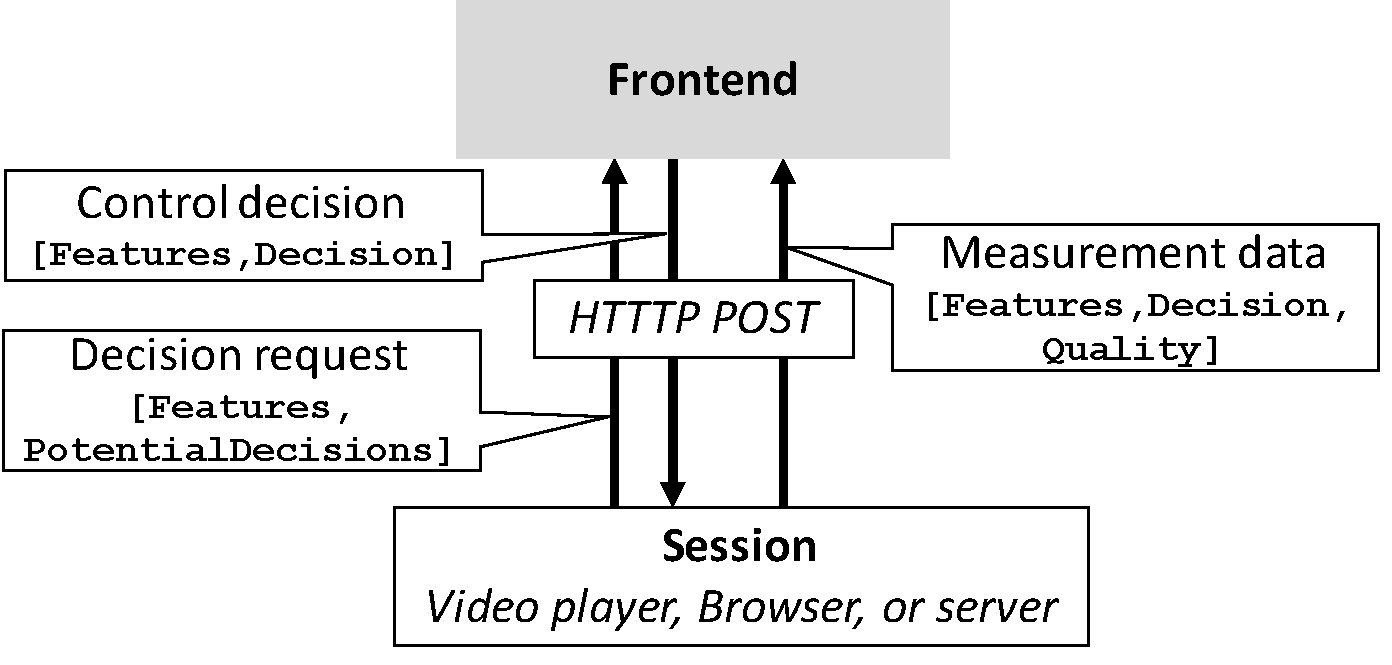
\includegraphics[width=0.6\textwidth]{figures/pytheas-impl-sep-api.pdf}
	\label{fig:impl-api}
}\\
%\hspace{-0.2cm}
\subfloat[Frontend]
{
        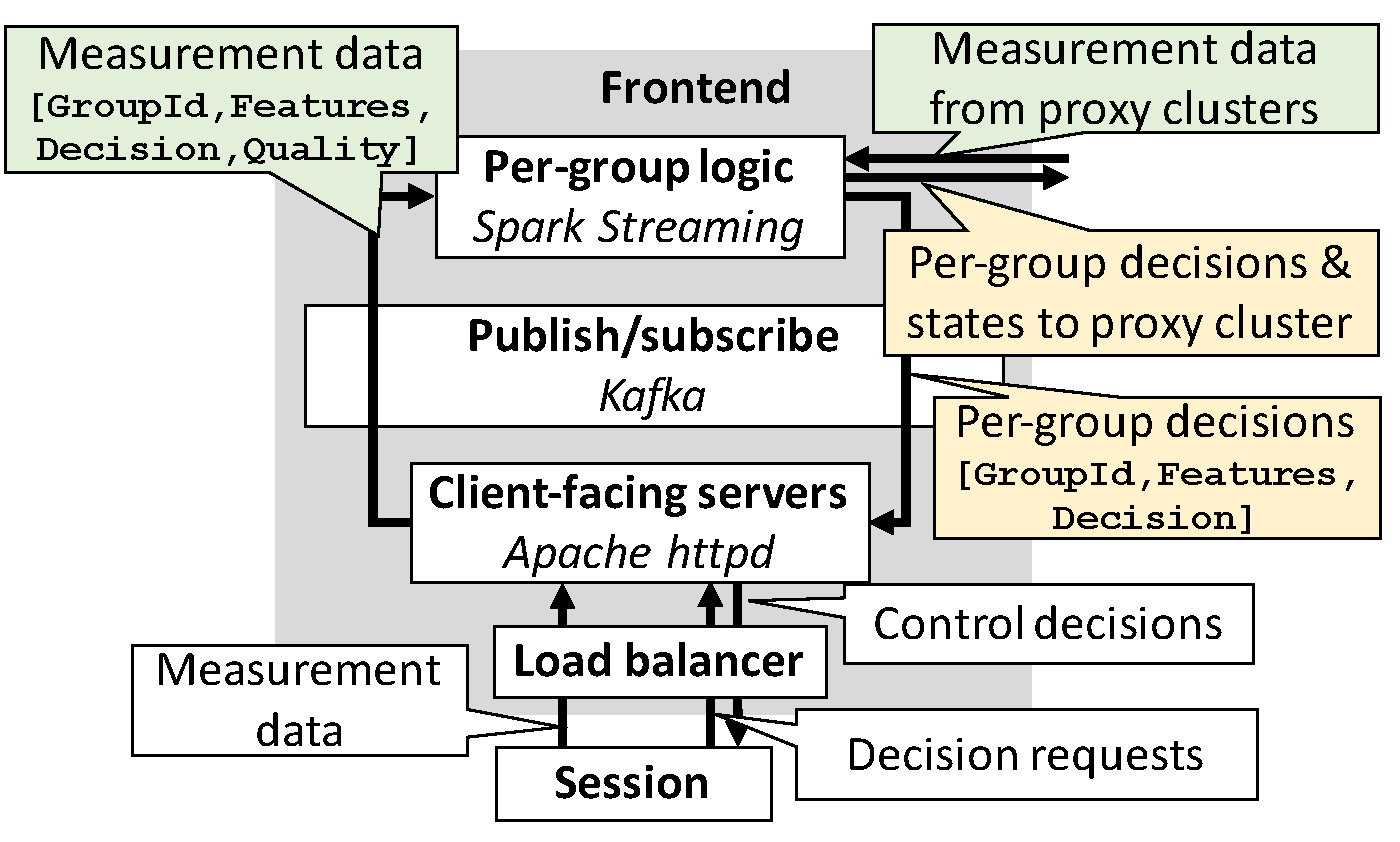
\includegraphics[width=0.6\textwidth]{figures/pytheas-impl-sep-frontend.pdf}
	\label{fig:impl-frontend}
}\\
%\hspace{-0.2cm}
\subfloat[Backend]
{
        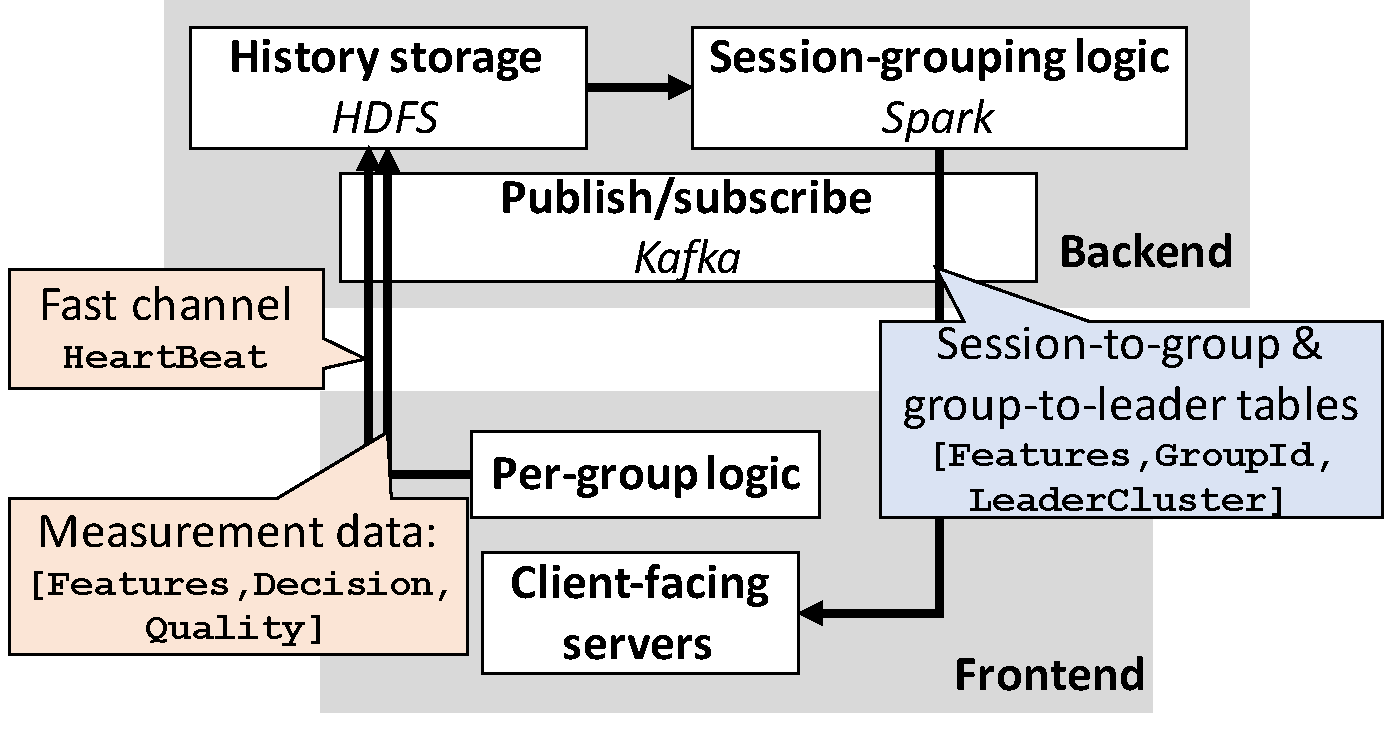
\includegraphics[width=0.6\textwidth]{figures/pytheas-impl-sep-backend.pdf}
	\label{fig:impl-backend}
}
%\hspace{-0.5cm}
%\vspace{-0.2cm}
\caption{Key components and interfaces of \name implementation.}
%\vspace{-0.4cm}
\label{fig:impl-overview}
\end{figure*}


%This section present the key details in implementation, and some lessons we learned in implementing the system.
%Since the key difference between \name and C3 is that the per-group control logic now resides in the frontend cluster (see \Section\ref{sec:system}), we will focus on the implementation of frontend clusters. 
%This section begins with a basic implementation of the two loops of \name, namely per-group control and session grouping,  as described in previous sections.
%We then identify the performance bottlenecks of this basic implementation and how we improved them.
\name is open source ($\approx$ 10K lines of code across Java, python,
and PHP) and can be accessed at~\cite{ddn-source}.  Next, we describe the APIs
for applications to integrate with \name, and then describe the implementation
of frontend and backend, as well as optimizations we used to remove \name's performance
bottlenecks. 

%\tightsubsection{Basic implementation}

\mypara{\name APIs}
Application sessions communicate with \name through two APIs
(Figure~\ref{fig:impl-frontend}): One for requesting control decisions, one for
uploading measurement data.  Both are implemented as standard HTTP POST
messages.  The session features are encoded in
the data field of the POST message.
\name also needs content providers to provide the schema of the message that 
 sessions send to the \name frontend, as well as a list of potential decisions.
Content providers may also provide QoE models that compute QoE metrics from 
the raw quality measurements sent by sessions.

%\vyas{APIs for providers?}

\mypara{Frontend}
Figure~\ref{fig:impl-frontend} shows the key components and interfaces of a
frontend cluster.  When a session sends a control request to \name, the request
will be received by one of the client-facing servers run by Apache
httpd~\cite{httpd}.  The server processes the request with a PHP script, which
first maps the session to a group and its leader cluster by matching
the session features with the session-to-group and group-to-leader tables.
Then the server queries the \mab
logic of the group (Section~\ref{subsec:per-group}), for the most up-to-date
decision of the group, and finally returns the decision to the session.  The
script to process the measurement data uploaded by a session is similar; a
client-facing server maps it to a group, and then forwards it to the per-group
\mab logic. The per-group \mab
logic is a Spark Streaming~\cite{sparkstreaming} program. It maintains a
key-value map (a Spark RDD) between group identification and the per-group \mab states (e.g., most recent decisions),
and updates the states every second by the most recent measurement data in one
MapReduce operation.  
 The communication between these processes is through
Kafka~\cite{kafka}, a distributed publish/subscribe service.  
We used Apache httpd, Spark Streaming, and Kafka, mainly
because they are horizontally scalable and highly resilient to failures of
individual machines.

While the above implementation is functionally sufficient, we observed that 
 the frontend throughput if implemented as-is is low. Next, we discuss 
 the optimizations to overcome the performance bottlenecks.
\begin{itemize}
\item{\em Separating logic from client-facing servers:}
When a client-facing server queries the per-group control logic, the client-facing server is effectively blocked, which significantly reduces the throughput of client-facing servers.
To remove this bottleneck, we add an intermediate process in each client-facing server to decouple querying control logic from responding requests.
It frequently (by default every half second) pulls the fresh decision of each group from per-group logic and writes the decision in a local file of the client-facing server. 
Thus, the client-facing server can find the most up-to-date decisions from local cache without directly querying the control logic.
\item{\em Replacing features with group identifier:}
We found that when the number of session features increases, Spark Streaming has significantly lower throughput as it takes too long to copy the new measurement data from client-facing servers to Kafka and from Kafka to RDDs of Spark Streaming.
This is avoidable, because once the features are mapped to a group by the client-facing servers, the remaining operations (updating and querying per-group logic) are completely feature-agnostic, so we can use group ID as the group identifier and remove all features from messages. 
%This significantly increases the Spark Streaming throughput (see Figure~\ref{fig:eval-optimization-sparkstreaming})
\end{itemize}


\mypara{Backend}
%Session grouping involves both frontend and backend.
Figure~\ref{fig:impl-backend} shows the key components and interfaces of the backend cluster.
Once client-facing servers receive the measurement data from sessions, they will forward the measurement data to the backend cluster.
On receiving these measurement data, the backend stores them in an HDFS for history data, and periodically (by default every 10 minutes) runs the session-grouping logic (Section~\ref{subsec:grouping}) as a Spark~\cite{spark} job to learn the session-group mapping and group-cluster mapping from the stored history data.
These tables are sent to each frontend through Kafka, so that the future messages (requests and measurement data) from sessions will be matched against new tables.
%\cameraremove{To implement the fast channel used for flash crowd detection, each frontend cluster maintains workload statistics and sends them to the backend every 5 seconds. 
%On receiving the data, the backend will then run a simple logic to detect flash crowd (\Section\ref{subsec:flashcrowd}) every 10 seconds.}
In addition, to detect failures of frontend clusters, each frontend cluster sends a small heartbeat message to the backend cluster every 5 seconds.




%\tightsubsection{Performance optimization}
%\label{subsec:optimization}
%
%While this basic implementation offers all functionalities, we found that the frontend throughput could be extremely low.
%This is caused by two bottlenecks which can be alleviated with simple optimization.

%\myparatight{Simplifying session-to-group lookup}
%We used PHP to process requests for its speed and support for runtime edits, but when the number of groups in the session-to-group table becomes too large, this will create a performance bottleneck.
%%Web servers today use scripting languages, such as php, to allow edits at runtime. 
%While this is fine in common cases, we need scripting code to look up a table that could have tens of thousands entries (i.e., groups), and this creates a performance bottleneck.
%In fact, we see throughput drops significantly when the number of groups exceeds certain critical threshold, typically about one thousand.
%We address this bottleneck by dividing all groups into several ``blocks'', so that the number of groups in block is lower than the threshold.
%%, and the total number of blocks is far less than the threshold.
%Each server now first maps a session to a block, and then looks up only the groups in this block.
%As a result, we can achieve the same throughput to a web server without any lookup operation (see Figure~\ref{fig:eval-optimization-throughput-blocklookup}) at little cost on processing time (two lookups instead of one).

%\myparatight{Separating logic from client-facing servers}
%In the basic implementation, to answer each request, the client-facing server needs to query the per-group control logic, during which the client-facing server will be effectively blocked, and significantly increasing the response time of each request.
%To remove this block, we introduce an intermediate process in each client-facing server to split decision updates from request responding.
%It pulls the fresh decision of each group from Kafka on a high frequency (by default every half second), but not on per request base, and writes the decision in a local file. 
%As a result, the client-facing server can return decisions by a simple cache lookup operation, while still preserving the desirable freshness of decisions.
%
%\myparatight{Replacing features with group identifier}
%We found that when we increase the number of session features, Spark Streaming will have significantly lower throughput because it takes too long for Spark Streaming to copy the data out from Kafka and store in memory.
%This is avoidable, because once the features are mapped to a group by the client-facing servers, the rest operations (updating and querying per-group logic) are completely feature-agnostic.
%Thus, once the client-facing servers map feature to a group, we will use group as the identifier and remove features from the message. 
%This significantly increases the Spark Streaming throughput (see Figure~\ref{fig:eval-optimization-sparkstreaming})
%, and also reduce the bandwidth consumption between frontend clusters (Figure~\ref{fig:eval-bandwidth}) (although features have to be sent to the backend for learning critical features and regrouping). 














\section{Evaluation}
\label{sec:pytheas:eval}


To evaluate \name, we run our prototype~\cite{ddn-source} across
multiple instances in CloudLab~\cite{cloudlab}.  Each instance is a physical
machine that has 8 cores (2.4 GHz) and 64GB RAM.  These instances are grouped 
 to form two frontend clusters and one backend
cluster (each includes 5 to 35 instances).  
This testbed is an end-to-end implementation of \name described in
Section~\ref{sec:pytheas:impl}\footnote{\name can use standard solutions such as DNS redirection
to map clients to frontend clusters, and existing load balancing mechanisms provided by the host
cloud service to select a frontend server instance for each client.}.


By running trace-driven evaluation and microbenchmarks on this testbed deployment, we show that:
\begin{packeditemize}
\item In the use case of video streaming, Pytheas improves the mean QoE by up to 6-31\% and the 90th percentile QoE by 24-78\%,
compared to a prediction-based baseline (Section~\ref{sec:eval:usecase}).  
\item \name is horizontally scalable and has similar low response delay to existing prediction-based systems  (Section~\ref{sec:eval:scale}).
\item \name can tolerate failures on frontend clusters by letting  clients fall back to local logic and rapidly recovering lost states from
 other frontends (Section~\ref{sec:eval:fail}).
\end{packeditemize}



%\myparatight{Micro-benchmark of performance}


\subsection{End-to-End Evaluation}
\label{sec:eval:usecase}

\mypara{Methodology}
To demonstrate the benefit of \name on improving QoE, we use a real-world trace of 8.5 million video sessions collected from a major video streaming sites in US over a 24-hour period. Each video session can choose one of two CDNs.
The sessions are replayed in the same chronological order as in the trace.
%, thereby allowing \name to gain knowledge as it goes along using newer QoE measurement. 
We call a group of sessions a {\em unit} if they match values on AS, city, connection type, player type and content name.\footnote{The notion of unit is used to ensure statistical confidence of QoE evaluation, and is not used in \name.}
 We assume that when a video session is assigned to a CDN, its QoE would be the same to the QoE of a session that is randomly sampled from the same unit who use the same CDN in the same one-minute time window.
For statistical confidence, we focus on the units which have at least 10 sessions on each CDN in each one-minute time windows for at least ten minutes. 
We acknowledge that our trace-driven evaluation has constraints similar to the related work, such as the assumption that QoE in a small time window is relatively stable in each unit (e.g.,~\cite{via}) and a small decision space (e.g.,~\cite{cfa}).

For each video session in the dataset, we run a DASH.js video player~\cite{dashjs}, which communicates with \name using the API described in Figure~\ref{fig:impl-api}. To estimate the QoE of a video session, the video player does not stream video content from the selected CDN. Instead, it gets the QoE measurement from the dataset as described above.

We use CFA~\cite{cfa} as the prediction-based baseline. It is implemented based on~\cite{cfa}.
CFA updates QoE prediction in the backend every minute, 
and trains critical features every hour.  
The frontend clusters run a simple decision-making algorithm -- for 90\% sessions,
it picks the decision that has the best predicted QoE, and for
the rest sessions, it randomly assigns them to a CDN.

We consider two widely used video QoE metrics~\cite{sigcomm11,cfa}: join time (the start-up delay of a video session), and buffering ratio (the fraction of session duration spent on rebuffering).
 We define improvement of \name for a particular unit at $t$-th minute by
  $\mathit{Improve}_{\mathit{\name}}(t)=\frac{Q_{CFA}(t)-Q_{\mathit{\name}}(t)}{Q_{CFA}(t)}$, where $Q_{\mathit{\name}}(t)$ and $Q_{CFA}(t)$ are the average QoE of \name in $t$-th minute and that of the baseline, respectively. 
Since we prefer smaller values on both metrics, a positive 
 value means  \name has better QoE.
%To highlight \name's improvement over the baseline in different units, 
%we define the mean improvement of \name for a unit by $\frac{1}{T}\sum_{t=1}^{T}\frac{Q_{CFA}(t)-Q_{Polis}(t)}{Q_{CFA}(t)}$, 
%Similarly, we can define 90 percentile improvement of each unit.
%In the rest of the section, we consider the \name improvement in these two metrics.


\begin{figure}[t!]
\captionsetup[subfigure]{justification=centering,farskip=-1pt,captionskip=5pt}
\centering
%\hspace{-0.5cm}
\subfloat[Join time]
{
        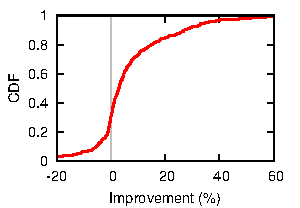
\includegraphics[width=0.45\textwidth]{figures/pytheas-Eval-overall-quality-shijie-2-jointime-cdf.pdf}
	\label{fig:eval-overall-quality-jointime}
}
%\hspace{-0.4cm}
\subfloat[Buffering ratio]
{
        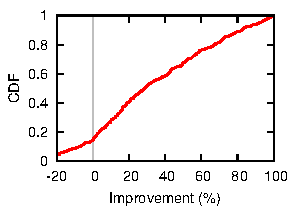
\includegraphics[width=0.45\textwidth]{figures/pytheas-Eval-overall-quality-shijie-2-bufratio-cdf.pdf}
	\label{fig:eval-overall-quality-bufratio}
}
%\hspace{-0.5cm}
%\vspace{-0.2cm}
\caption{Distribution of improvement of \name over the prediction-based baseline.}
%\vspace{-0.2cm}
\label{fig:eval-overall-quality}
\end{figure}

\mypara{Overall improvement} Figure~\ref{fig:eval-overall-quality} shows
the distribution of improvement of \name across all sessions.  We can see that
the mean improvement is 6\% for join time and 31\% for buffering ratio, and the
90th percentile improvement is 24\% for join time and 78\% for buffering ratio.
To put these numbers in context, prior studies 
show a 1\% decrease in buffering can lead to more than a 3-minute increase 
in expected viewing time~\cite{sigcomm11}.
Note that \name is not better than the baseline on every single 
session, because the \mab process inherently uses a
(dynamic) fraction of traffic to explore suboptimal decisions.
% Next, we evaluate two scenarios where \name has greater improvement.


\begin{figure}[t!]
\captionsetup[subfigure]{justification=centering,farskip=-1pt,captionskip=0pt}
\centering
%\hspace{-0.5cm}
\subfloat[Join time]
{
        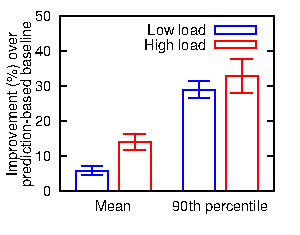
\includegraphics[width=0.45\textwidth]{figures/pytheas-Eval-loadeffect-shijie-jointime-2.pdf}
	\label{fig:eval-loadeffect-jointime}
}
%\hspace{-0.4cm}
\subfloat[Buffering ratio]
{
        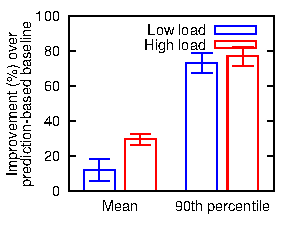
\includegraphics[width=0.45\textwidth]{figures/pytheas-Eval-loadeffect-shijie-bufratio-2.pdf}
	\label{fig:eval-loadeffect-bufratio}
}
%\hspace{-0.5cm}
%\vspace{-0.2cm}
\caption{Improvement in presence of load effect.}
%\vspace{-0.cm}
\label{fig:eval-loadeffect}
\end{figure}

%\begin{figure}[t!]
%\centering
%\includegraphics[width=0.35\textwidth]{figures/motivation/Eval-loadeffect.pdf}
%\vspace{-0.2cm}
%\tightcaption{Impact of load effect on the improvement of \name}
%\label{fig:eval-loadeffect}
%\end{figure}

\mypara{Impact of load-induced QoE degradation}
%We also want to understand the impact of load effect on the benefit of \name.
%To that end, we consider the units whose sessions could have significantly degraded quality when one CDN has a load over certain threshold.
We consider the units where QoE of a CDN could significantly degrade when most sessions of the unit are assigned to use the same CDN.
We assume that the QoE of a session when using a CDN under a given load (defined by the number of sessions assigned to the CDN in one minute) is the same to the QoE of a session randomly chosen in the dataset which uses the same CDN when the CDN is under a similar load. 
Figure~\ref{fig:eval-loadeffect} shows that the improvement of \name when the number of sessions is large enough to overload a CDN is greater than the improvement when the number of sessions is not large enough to overload any CDN.
%We can see that \name has a greater improvement when load-induced QoE degradation is possible. 
This is because the prediction-based baseline could overload a CDN when too many sessions are assigned to the same CDN before CFA updates the QoE prediction, whereas \name avoids overloading CDNs by updating its decisions in real time.

%\cameraremove{\myparatight{Handling flashcrowd}}
%\cameraremove{Finally, we consider when flashcrowd can lead to QoE degradation on certain video object.
%Since this is a VoD dataset, flashcrowd is relatively rare. 
%So we created synthetic trace by adding many video sessions who join at the same moment to watch certain object so that it creates load-induced QoE degradation on CDNs' performance on this particular object.
%Figure~\ref{fig:eval-flashcrowd} shows that \name has greater improvement after a flashcrowd happens. 
%This is because \name can regroup based on real-time feedback on workload.
%}
%
%\cameraremove{
%\camera{Finally, we consider a case where the sessions of a certain video object increase dramatically in a very short period of time, which simulates a flash-crowd event.
%To this end, we created a synthetic trace by adding many video sessions at the same moment to watch the same video object, and this sudden increase in load could led to QoE degradation on CDNs' performance on this particular object. 
%We assume that the sessions of this video object is in the same session group, which in real world may require additional logic to ensure (see \Section\ref{sec:discuss}).
%Figure~\ref{fig:eval-flashcrowd} shows that \name achieves better QoE than CFA, because \name can immediately adjust CDN selection to cope with sudden load increase based on real-time feedback, while CFA cannot react fast enough.}
%}

%Finally, \name should also be robust to flashcrowd. 
%Figure~\ref{fig:eval-flashcrowd} shows the behavior of \name in the example of Figure~\ref{subfig:problem-of-slow:flash}. 
%We can see that because \name detects sharp raise in viewership of object X as soon as it appears, it can react by creating a new group for the session watching X and make different decisions independently to other sessions. 


%\cameraremove{
%\begin{figure}[t!]
%\captionsetup[subfigure]{justification=centering,farskip=-1pt,captionskip=0pt}
%\centering
%\hspace{-0.5cm}
%\subfloat[Join time]
%{
%        \includegraphics[width=0.25\textwidth]{figures/motivation/Eval-flashcrowd-shijie-jointime-2.pdf}
%	\label{fig:eval-flashcrowd-jointime}
%}
%\hspace{-0.4cm}
%\subfloat[Buffering ratio]
%{
%        \includegraphics[width=0.25\textwidth]{figures/motivation/Eval-flashcrowd-shijie-bufratio-2.pdf}
%	\label{fig:eval-flashcrowd-bufratio}
%}
%\hspace{-0.5cm}
%\vspace{-0.2cm}
%\tightcaption{Improvement in presence of flash crowd}
%%\vspace{-0.2cm}
%\label{fig:eval-flashcrowd}
%\end{figure}
%}

\mypara{Contribution of \name ideas}
Having shown the overall benefit of \name, we now evaluate the contribution of different components of \name: (1) \mab;
 (2)  real-time update; and  (3) grouping. 
We replace certain pieces of \name by baseline solutions and compare their QoE with \name's QoE.
 Specifically, for (1), we replace the per-group \mab logic by CFA's decision-making logic; 
for (2), we run  \name with  data of one-minute staleness; and for (3), 
 we run the same \mab process over all sessions, rather than on per-group basis.
%three hypothetical baselines, each of which differs to \name only in one aspect and thus highlights the importance of one aspect of \name.
%\begin{packeditemize}
%\item Benefit of ``\mab'' is shown by ``Real-time CFA'' which differs to \name only in that it runs CFA logic, instead of \mab, for per-group control.
%\item Benefit of ``real-time'' is shown by ``Stale \mab'' which differs to  \name only in that it uses data of one minute stale. One can think of it as a centralized way of running \mab by the backend with stale data~\cite{velox-cidr}. 
%\item Benefit of ``grouping'' is shown by ``Global \mab'' which differs to \name in that it runs the same \mab process over all sessions, rather than on per-group base.
%\end{packeditemize
Figure~\ref{fig:eval-separate} shows the improvement of \name over each baseline, and it shows that each of these ideas contributes a nontrivial improvement to \name; about 10-20\% improvement on average QoE and 15-80\% on the 90th percentiles. 

%First, to highlight the benefit of ``\mab'', we compare \name with a hypothetical baseline called {\em real-time CFA}, which differs to \name only in that it runs CFA logic for per-group control.
%Second, to highlight the benefit of ``real-time'', we compare \name with a hypothetical baseline called {\em stale \mab}, which differs 

%%%% prediction -> real-time prediction -> real-time E2
%%%% global stale e2 -> global real-time e2 -> group-based real-time E2

%we consider a hypothetical baseline called {\em real-time CFA}, which updates CFA QoE prediction at the same frequency to \name (i.e., every second)\footnote{Real-time CFA is feasible in \name, but is impractical in the original CFA implementation since it could not update prediction in real time.}. 
%Figure~\ref{fig:eval-separate} compares the mean and tail improvements of real-time CFA and real-time \mab (\name). 
%We can see that the improvement of real-time CFA is great, but real-time \mab has a much larger improvement, especially on the tails. 
%This suggests that both ``real-time'' and ``\mab'' are needed to achieve full potential of data-driven optimization.



\begin{figure}[t!]
\captionsetup[subfigure]{justification=centering,farskip=-1pt,captionskip=0pt}
\centering
%\hspace{-0.5cm}
\subfloat[Join time]
{
        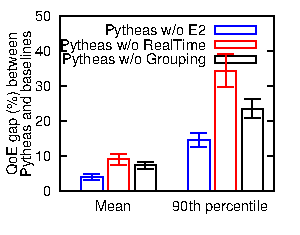
\includegraphics[width=0.45\textwidth]{figures/pytheas-Eval-OtherEE-shijie-jointime-2.pdf}
	\label{fig:eval-separate-jointime}
}
%\hspace{-0.4cm}
\subfloat[Buffering ratio]
{
        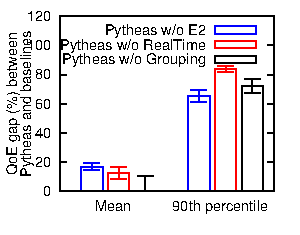
\includegraphics[width=0.45\textwidth]{figures/pytheas-Eval-OtherEE-shijie-bufratio-2.pdf}
	\label{fig:eval-separate-bufratio}
}
%\hspace{-0.5cm}
%\vspace{-0.2cm}
\caption{Factor analysis of \name ideas} %Separating the benefit of ``\mab'', ``real time'', and ``groupping''.}
%\vspace{-0.2cm}
\label{fig:eval-separate}
\end{figure}



\subsection{Microbenchmarks}

\label{sec:eval:scale}

%In addition to the small-scale testbed for trace-driven emulation, 
We create micro-benchmarks to evaluate the scalability and bandwidth
consumption of \name, as well as the benefits of various performance optimizations (Section~\ref{sec:pytheas:impl}).




\subsubsection{Scalability}
\myparatight{Frontend}
Figure~\ref{fig:eval-frontend-scalability} shows the maximum number of sessions that can be served in one second, while keeping the update interval of per-group logic to be one second. 
Each session makes one control request and uploads QoE measurement once. Each group has the same amount of sessions.
The size of control request message is 100B. We run Apache Benchmark~\cite{apache-benchmarking} for 20 times and report the average throughput.
We can see that the throughput is almost horizontally scalable to more frontend server instances. 
%Moreover, \name achieves almost the same throughput to a frontend cluster with the same resource that does not need to run the per-group control logic (e.g., a C3 frontend cluster).
 While  the number of groups does impact the performance of frontend cluster, it is only to a limited extent; throughput of handling 10K groups is about 10\% worse than that of handling one group.

Next, we evaluate the performance optimizations described in Section~\ref{sec:pytheas:impl}.
We use a frontend cluster of 32 instances.
Figure~\ref{fig:eval-optimization-frontend} shows that by separating \mab logic from client-facing servers, we can achieve 8x higher throughput, because each request reads cached decisions, which are still frequently updated.
By replacing features by group identifiers, we can further increase throughput  by 120\%, because we can copy less data from client-facing servers to the servers running \mab logic.
%As a result, the frontend throughput is as high as if all instances are used as web servers without any control logic.
Note these results do not merely show the scalability of Spark Streaming or web servers; they show that our implementation of \name introduces minimal additional cost, and can fully utilize existing data analytics platforms.

%We use one client-facing server instance, and set the request message to be 100B.

%Figure~\ref{fig:eval-optimization-frontend} shows that while unoptimized session-to-group lookup has significantly lower throughput with increasing numbers of groups, block-based lookup can achieve almost the same throughput to a simple web server that does no lookup. 
%Using the same setup, we also found that by separating query of control logic from the process of responding each request, client-facing server throughput is 800\% higher than if each request is processed by querying the control logic (not shown in figure).
%Finally, we increase the request message size, and show in Figure~\ref{fig:eval-optimization-sparkstreaming} that the throughput of per-group logic is very sensitive to the size of session features, and by replacing session features with group identifiers and thus keeping the message size constant, per-group logic can maintain high throughput independently with the message size.


\begin{figure}[t!]
\captionsetup[subfigure]{justification=centering,farskip=-1pt,captionskip=5pt}
\centering
%\hspace{-0.5cm}
\subfloat[Frontend]
{
        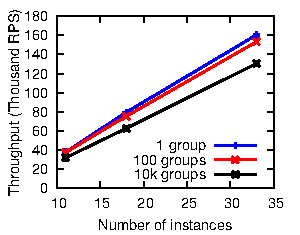
\includegraphics[width=0.45\textwidth]{figures/pytheas-Eval-scalability-frontend.pdf}
	\label{fig:eval-frontend-scalability}
}
%\hspace{-0.4cm}
\subfloat[Backend]
{
        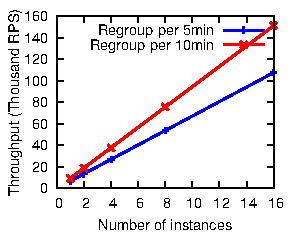
\includegraphics[width=0.45\textwidth]{figures/pytheas-Eval-scalability-backend.pdf}
	\label{fig:eval-backend-scalability}
}
%\hspace{-0.5cm}
%\vspace{-0.1cm}
\caption{\name throughput is horizontally scalable.}
%\vspace{-0.2cm}
\label{fig:scalability}
\end{figure}

\begin{figure}[t!]
\centering
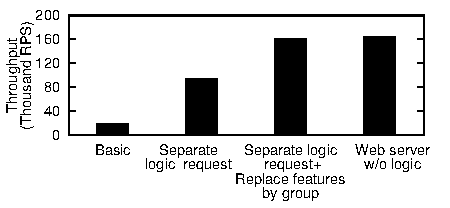
\includegraphics[width=0.6\textwidth]{figures/pytheas-Eval-optimization-separatelogic-replacingfeatures-bar.pdf}
%\vspace{-0.2cm}
\caption{Optimizations of frontend throughput.}
\label{fig:eval-optimization-frontend}
\end{figure}


\mypara{Backend}
Figure~\ref{fig:eval-backend-scalability} shows the maximum number of sessions that can be served in each second by a backend cluster, while keeping the completion time of session-grouping logic within 5 minutes or 10 minutes.
We see that the throughput is also horizontally scalable with more instances in the backend cluster. 

To put the scalability numbers of both frontend and backend in context, let us consider a content provider like YouTube which has 5 billion sessions per day~\cite{youtube-stats} (i.e., 57K sessions per second). 
%. , which is on average 3.5 million sessions per second. 
%the traffic is evenly spread over time, that is 57K sessions per second. 
\name can achieve this throughput using one frontend cluster of 18 instances and a backend cluster of 8 instances, which is a tiny portion compared to the sheer number of video servers (at least on the magnitude of hundreds of thousands~\cite{youtube-stats-2}).
This might make Spark Streaming and Kafka an overkill for \name, but the scale of data rate can easily increase by one to two magnitudes in real world, e.g., tens of GB/s; for instance, each video session can request tens of mid-stream decisions during an hour-long video, instead of an initial request.




\subsubsection{Bandwidth consumption}

Since the inter-cluster bandwidth could be costly~\cite{geode,iris}, we now evaluate the inter-cluster bandwidth consumption of \name. %especially when request message size is large, or when many sessions are not received by the leader clusters.
We consider one session group that has one proxy cluster and one leader cluster.

First, we evaluate the impact of message size. 
We set the fraction of sessions received by the proxy cluster to be 5\% of the group, and increase the request message size by adding more features. 
Figure~\ref{fig:eval-bandwidth-message} shows that the bandwidth consumption between the frontend clusters does not grow with larger message size, because the session features are replaced by group identifiers by the client-facing servers.
Only the bandwidth consumption between frontend and backend grows proportionally with the message size
but such overhead is inherent in existing data collection systems and is not caused by \name.

Next, we evaluate the impact of fraction of sessions received by the proxy cluster. 
We set the message size to be 400B, and change the fraction of sessions received by each proxy cluster.
Figure~\ref{fig:eval-bandwidth-message} shows that the bandwidth consumption between frontend clusters raises as more measurement data need to be forwarded from proxy to the leader cluster, but it is much smaller than the bandwidth consumption between frontend and backend.

%\jc{some words on further reducing the overhead?}


\begin{figure}[t!]
\captionsetup[subfigure]{justification=centering,farskip=-1pt,captionskip=5pt}
\centering
%\hspace{-0.5cm}
\subfloat[Impact of message size]
{
        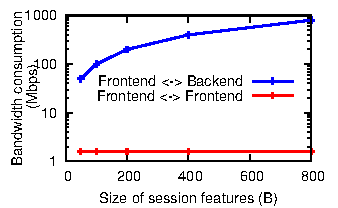
\includegraphics[width=0.45\textwidth]{figures/pytheas-Eval-bandwidth-message.pdf}
	\label{fig:eval-bandwidth-message}
}
%\hspace{-0.5cm}
\subfloat[Impact of \% sessions not in the leader cluster]
{
        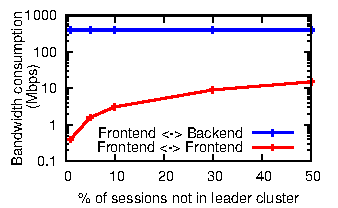
\includegraphics[width=0.45\textwidth]{figures/pytheas-Eval-bandwidth-fracproxy.pdf}
	\label{fig:eval-bandwidth-fracproxy}
}
%\hspace{-0.5cm}
%\vspace{-0.1cm}
\caption{Bandwidth consumption between clusters.}
%\vspace{-0.2cm}
\label{fig:eval-bandwidth}
\end{figure}



%\begin{figure}[t!]
%\captionsetup[subfigure]{justification=centering,farskip=-1pt,captionskip=5pt}
%\centering
%\hspace{-0.5cm}
%%\subfloat[Block-based group lookup]
%%{
%%        \includegraphics[width=0.25\textwidth]{figures/motivation/Eval-optimization-throughput-blocklookup.pdf}
%%	\label{fig:eval-optimization-throughput-blocklookup}
%%}
%%\hspace{-0.5cm}
%\subfloat[Separating logic from request responding]
%{
%        \includegraphics[width=0.25\textwidth]{figures/motivation/Eval-optimization-throughput-decoupled.pdf}
%	\label{fig:eval-optimization-throughput-decoupled}
%}
%\hspace{-0.5cm}
%\subfloat[Replacing features by group]
%{
%        \includegraphics[width=0.25\textwidth]{figures/motivation/Eval-optimization-sparkstreaming.pdf}
%	\label{fig:eval-optimization-sparkstreaming}
%}
%\hspace{-0.5cm}
%\vspace{-0.1cm}
%\tightcaption{Benefit of performance optimizations on throughput of frontend clusters.}
%%\vspace{-0.2cm}
%\label{fig:eval-bandwidth}
%\end{figure}



%Figure~\ref{fig:eval-optimization-throughput-decoupled} shows the benefit of separating logic from request responding on the throughput of  client-facing servers.
%We fixed the message size to be 100B and used one group.






\subsection{Fault Tolerance}
\label{sec:eval:fail}

Finally, we stress test the prototype under the condition that a leader frontend cluster fails. 
 We set up 10 video players, each of which can stream content from two CDNs. CDN1 has 5000ms join time and CDN2 has 1000ms join time. By default, the player's native logic chooses CDN1.
There are two frontend clusters, f1 and f2. 
The experiment begins with f1 being the leader cluster, and it loses connection at $t=25$.

Figure~\ref{fig:eval-fault-tolerance} shows the time-series of QoE of sessions that are mapped to each frontend clusters.
First, we see that the sessions mapped to f1 can fall back to the CDN chosen by the player's native logic, rather than crashing.
Second, right after f1 fails, f2 should still be able to give cached decision (made by f1 before it fails) to its sessions.
At $t=30$, the backend selects f2 as the new leader for the group. 
At the point, a naive way to restart per-group logic in the new leader is to start it from scratch, but this will lead to suboptimal QoE at the beginning (the dotted line between $t=30$ and $t=35$).
\name avoids this cold-start problem by keeping a copy of the per-group states in the proxy cluster. This allows the proxy cluster to recover the per-group control states without QoE degradation.




\begin{figure}[t!]
\centering
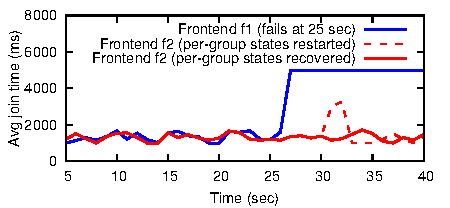
\includegraphics[width=0.6\textwidth]{figures/pytheas-Eval-fault-tolerance.pdf}
%\vspace{-0.2cm}
\caption{\name can tolerate loss of a frontend cluster by falling back to player native logic gracefully, and recovering the logic states in a new cluster.}
\label{fig:eval-fault-tolerance}
\end{figure}



%\section{Discussion}
\label{sec:pytheas:discuss}

\mypara{Handling flash crowds}
Flash crowds happen when many sessions join at the same time and cause part of the resources (decisions) to be overloaded.
While \name can handle load-induced QoE fluctuations that occur in individual groups, overloads caused by flash crowds are different, in that they could affect sessions in multiple groups. Therefore, those affected sessions need to be regrouped immediately, but \name does not support such real-time group learning. 
To handle flash crowds, \name needs a mechanism to detect flash crowds and create groups for the affected sessions in real time.

%\mypara{Use of active measurement}
%While our system relies entirely on passive QoE measurements as input of data-driven optimization, we see a new opportunity to augment the system with active measurements by orchestrating vantage points and controlled clients (e.g., Skype~\cite{via}) to establish fake traffic.
%These active measurement can be used to explore suboptimal decisions, thereby reducing the cost of \mab on real sessions. 
%One also needs to take into consideration the additional load due to these active measurements.


\mypara{Cost of switching decisions}
The current design of \name assumes there is little cost to switch the decision during the course of a session. 
While such assumption applies to today's DASH-based video streaming protocols~\cite{dash-standard}, other applications (e.g., VoIP) may have significant cost when switching decisions in the middle of a session, so the control logic should not too sensitive to QoE fluctuations.
Moreover, a content provider pays CDNs by 95th percentile traffic, so \name must carefully take the traffic distribution into account as well.
We intend to explore decision-making logic that is aware of these costs of switching decisions in the future.




\section{Related Work}
\label{sec:pytheas:related}


\mypara{Data-driven QoE optimization}
There is a large literature on using data-driven techniques to optimize QoE for a variety of applications,
%While the focus has traditionally been how to adapt to changing network conditions and resource availability based on information observed by the same session, e.g., video bitrate adaptation~\cite{huang2014buffer}, research and industry is increasingly relying on data of multiple sessions to inform QoE optimization for many applications, 
such as video streaming (e.g.,~\cite{c3,cfa}), web service (e.g.,~\cite{footprint,spand}), Internet telephony~\cite{rewan-hotnets2015,via}, cloud services (e.g.,~\cite{lacurts2014cicada}), and resource allocation (e.g.,~\cite{bao2015data}). 
Some recent work also shows the possibility of using measurement traces to extrapolate the outcome of new system configurations~\cite{mwt}.
%Its focus has traditionally been to infer and adapt to the changing network conditions based on information gathered from the same session~\cite{??} or same client~\cite{??}, such as adaptive bitrate algorithm in video~\cite{??} and cloud server selection~\cite{??}.
%Though such local adaptation approach has served us well for decades, it has limitations (e.g., hard to adapt initial decisions~\cite{cfa}).
%This motivates the recent, more data-driven approaches where application providers use client-side instrumentations and real-time telemetry to optimize individual session QoE with the visibility of many sessions, and we see adoption of this approach in many contexts, video streaming~\cite{??}, Internet telephony~\cite{??}, web service~\cite{??}, and cloud services~\cite{??}. 
Unlike these prediction-based approaches, we formulate QoE optimization as an real-time \mab process, and show that by avoiding measurement bias and enabling real-time updates, this new formulation achieves better QoE than prediction-based approaches.

% and in a variety of contexts, including network resource allocation~\cite{bao2016prediction,bao2015data}

%\cameraremove{
%\myparatight{Exploration and exploitation techniques}
%}
\mypara{Related machine learning techniques}
\mab is closely related to reinforcement learning~\cite{mab}, where most techniques, including the per-group \mab logic used in \name, are variants of the UCB1 algorithm~\cite{ucb1}, though other approaches (e.g.,~\cite{agarwal2014taming}) have been studied as well. 
%which has good empirical performance and enjoys theoretical guarantees, 
Besides \mab, \name also shares the similar idea of clustering with linear mixed models~\cite{mcculloch2001generalized}, where a separate model is trained for each cluster of data points.
%UCB variants that are particular relevant to this paper include those aims at contextual settings~\cite{cmab} and time varying rewards~\cite{besbes2014stochastic}.
While we  borrow  techniques from this rich literature~\cite{discounteducb,regressogram-ucb}, our contribution is to shed light on the link between QoE optimization and the techniques of \mab and clustering, to highlight the practical challenges of adopting \mab in network applications, and to show \idea as a practical way to solve these challenges.
Though there have been prior attempts to cast data-driven optimization as multi-armed bandit processes in specific applications (e.g.,~\cite{via}), they fall short of a practical system design.

\mypara{Geo-distributed data analytics}
%A key challenge of data-driven QoE optimization is 
%Most work on large-scale data analytics (e.g.,~\cite{zaharia2012resilient,velox-cidr}) assumes that data are available in the same data center.
Like \name, recent work~\cite{iris,jetstream,geode} also observes that for cost and legal considerations, many geo-distributed applications store client-generated data in globally distributed data centers. However, they focus on geo-distributed data analytics platforms that can handle general-purpose queries received by the centralized backend cluster.
In contrast, \name targets a different workload: data-driven QoE optimization uses a specific type of logic (i.e., \mab), but has to handle requests from millions of geo-distributed sessions in real time.



\section{Summary}
\label{sec:pytheas:summary}

%With increasing demands of user QoE and diverse operating
%conditions, application providers are on an inevitable
%trajectory to adopt data-driven techniques. 
While previous two chapters
have achieved impressive QoE improvement by formulating \ddn as a 
prediction process, they have key limitations
%However, existing prediction-based approaches have key limitations
that curtail the potential of data-driven optimization.
Drawing on a parallel from machine learning, we
argue that real-time exploration and exploitation is a better
abstraction for this domain. In designing Pytheas, we
addressed key practical challenges in applying real-time
E2 to network applications. Our key insight is a {\em group-based
E2} mechanism, inspired by the insight of persistent structures in
QoE-determining factors. We observe that application sessions sharing
the same features can be grouped so that we can run
E2 at a coarser per-group granularity. Using an end-to-end
implementation and proof-of-concept deployment of
Pytheas in CloudLab, we showed that Pytheas improves
video quality over state-of-the-art prediction-based system
by 6-31\% on mean, and 24-78\% on tail QoE.




